%%%%%%%%%%%%%%%%%%%%%%%%%%%%%%%%%%%%%%%%%%%%%%%%%%%%%%%%%%%%%%%%%%%%%
%% This is a (brief) model paper using the achemso class
%% The document class accepts keyval options, which should include
%% the target journal and optionally the manuscript type.
%%%%%%%%%%%%%%%%%%%%%%%%%%%%%%%%%%%%%%%%%%%%%%%%%%%%%%%%%%%%%%%%%%%%%
\documentclass[journal=jpcbfk,manuscript=article]{achemso}

%\documentclass[english,aps,preprint,pre,floatfix,nofootinbib,showpacs,showkeys]{revtex4-1}
%%%%%%%%%%%%%%%%%%%%%%%%%%%%%%%%%%%%%%%%%%%%%%%%%%%%%%%%%%%%%%%%%%%%%
%% Place any additional packages needed here.  Only include packages
%% which are essential, to avoid problems later. Do NOT use any
%% packages which require e-TeX (for example etoolbox): the e-TeX
%% extensions are not currently available on the ACS conversion
%% servers.
%%%%%%%%%%%%%%%%%%%%%%%%%%%%%%%%%%%%%%%%%%%%%%%%%%%%%%%%%%%%%%%%%%%%%
\usepackage[version=3]{mhchem} % Formula subscripts using \ce{}

\SectionNumbersOn

%include hyperlinks to figures
%\documentclass{article}
\usepackage{graphicx}
\usepackage[%  
    colorlinks=true,
    pdfborder={0 0 0},
    linkcolor=black,
    citecolor=black,
    urlcolor=black
]{hyperref}

\usepackage{amsmath}
\usepackage{amssymb}
\usepackage{color}
\usepackage{CJK}
\usepackage{framed}
\usepackage{achemso}

%\usepackage[hidelinks]{hyperref}
%\usepackage{algpseudocode}
%\algdef{SE}[DOWHILE]{Do}{doWhile}{\algorithmicdo}[1]{\algorithmicwhile\ #1}

\usepackage[scaled=0.85]{beramono}
\usepackage[T1]{fontenc}
\usepackage{changepage}
\usepackage{mathrsfs}
\usepackage{comment}
\usepackage[normalem]{ulem}
\usepackage{algorithm}
\usepackage{subfig}
\usepackage{algpseudocode}

%%%%%%%%%%%%%%%%%%%%%%%%%%%%%%%%%%%%%%%%%%%%%%%%%%%%%%%%%%%%%%%%%%%%%
%% If issues arise when submitting your manuscript, you may want to
%% un-comment the next line.  This provides information on the
%% version of every file you have used.
%%%%%%%%%%%%%%%%%%%%%%%%%%%%%%%%%%%%%%%%%%%%%%%%%%%%%%%%%%%%%%%%%%%%%
%%\listfiles

%%%%%%%%%%%%%%%%%%%%%%%%%%%%%%%%%%%%%%%%%%%%%%%%%%%%%%%%%%%%%%%%%%%%%
%% Place any additional macros here.  Please use \newcommand* where
%% possible, and avoid layout-changing macros (which are not used
%% when typesetting).
%%%%%%%%%%%%%%%%%%%%%%%%%%%%%%%%%%%%%%%%%%%%%%%%%%%%%%%%%%%%%%%%%%%%%

\makeatletter
    \setlength\@fptop{0\p@}
\makeatother

%\newcommand*\mycommand[1]{\texttt{\emph{#1}}}

%\newcommand{\state}[1]{$\mathcal{S}_{#1}$}
%\newcommand{\Expect}[1]{\mathrm{E}\left[#1\right]}
%\newcommand{\norm}[1]{\left\lVert#1\right\rVert}

\newcommand*{\rood}[1]{{\color{red}{#1}}}
%\newcommand*{\blauw}[1]{\textcolor{blue}{#1}}
\newcommand*{\blauw}[1]{{#1}}

%\newcommand*{\addref}[1]{\textcolor{red}{\{ADD REF: #1\}}}
%\newcommand*{\noter}[1]{\textcolor{red}{[[#1]]}}		% notes 
%\newcommand*{\noter}[1]{}					% notes off
%\newcommand*{\noteb}[1]{\textcolor{blue}{[[#1]]}}		% notes 

%\usepackage[draft]{todonotes}   % notes shown
%\usepackage[disable]{todonotes} % notes hidden



%%%%%%%%%%%%%%%%%%%%%%%%%%%%%%%%%%%%%%%%%%%%%%%%%%%%%%%%%%%%%%%%%%%%%
%% Meta-data block
%% ---------------
%% Each author should be given as a separate \author command.
%%
%% Corresponding authors should have an e-mail given after the author
%% name as an \email command. Phone and fax numbers can be given
%% using \phone and \fax, respectively; this information is optional.
%%
%% The affiliation of authors is given after the authors; each
%% \affiliation command applies to all preceding authors not already
%% assigned an affiliation.
%%
%% The affiliation takes an option argument for the short name.  This
%% will typically be something like "University of Somewhere".
%%
%% The \altaffiliation macro should be used for new address, etc.
%% On the other hand, \alsoaffiliation is used on a per author basis
%% when authors are associated with multiple institutions.
%%%%%%%%%%%%%%%%%%%%%%%%%%%%%%%%%%%%%%%%%%%%%%%%%%%%%%%%%%%%%%%%%%%%%
\author{Michael S. Jones}
\affiliation{%
  Pritzker School of Molecular Engineering, %
  The University of Chicago, %
  5640 South Ellis Avenue, Chicago, Illinois 60637, United States%
}

\author{Brennan Ashwood}
\affiliation{%
  Department of Chemistry, Institute for Biophysical Dynamics, and James Franck Institute, %
  The University of Chicago, %
  929 East 57th Street, Chicago, Illinois 60637, United States%
}

\author{Andrei Tokmakoff}
\affiliation{%
  Department of Chemistry, Institute for Biophysical Dynamics, and James Franck Institute, %
  The University of Chicago, %
  929 East 57th Street, Chicago, Illinois 60637, United States%
}

\author{Andrew L. Ferguson}
\email{andrewferguson@uchicago.edu}
\affiliation{%
  Pritzker School of Molecular Engineering, %
  The University of Chicago, %
  5640 South Ellis Avenue, Chicago, Illinois 60637, United States%
}


%\author{Kay T. Finally}
%\affiliation[Unknown University]
%{Department of Chemistry, Unknown University, Unknown Town}
%\alsoaffiliation[Second University]
%{Department of Chemistry, Second University, Nearby Town}

%%%%%%%%%%%%%%%%%%%%%%%%%%%%%%%%%%%%%%%%%%%%%%%%%%%%%%%%%%%%%%%%%%%%%
%% The document title should be given as usual. Some journals require
%% a running title from the author: this should be supplied as an
%% optional argument to \title.
%%%%%%%%%%%%%%%%%%%%%%%%%%%%%%%%%%%%%%%%%%%%%%%%%%%%%%%%%%%%%%%%%%%%%
\title[]{Determining sequence-dependent DNA oligonucleotide hybridization and dehybridization mechanisms using coarse-grained molecular simulation, Markov state models, and infrared spectroscopy}


%%%%%%%%%%%%%%%%%%%%%%%%%%%%%%%%%%%%%%%%%%%%%%%%%%%%%%%%%%%%%%%%%%%%%
%% Some journals require a list of abbreviations or keywords to be
%% supplied. These should be set up here, and will be printed after
%% the title and author information, if needed.
%%%%%%%%%%%%%%%%%%%%%%%%%%%%%%%%%%%%%%%%%%%%%%%%%%%%%%%%%%%%%%%%%%%%%
%\abbreviations{IR -- infrared, NMR -- nuclear magnetic resonance, UV -- ultraviolet}
%\keywords{Takens}

\begin{document}
%%%%%%%%%%%%%%%%%%%%%%%%%%%%%%%%%%%%%%%%%%%%%%%%%%%%%%%%%%%%%%%%%%%%%
%% The manuscript does not need to include \maketitle, which is
%% executed automatically.  The document should begin with an
%% abstract, if appropriate.  If one is given and should not be, the
%% contents will be gobbled.
%%%%%%%%%%%%%%%%%%%%%%%%%%%%%%%%%%%%%%%%%%%%%%%%%%%%%%%%%%%%%%%%%%%%%

\newpage

\begin{abstract} % 250 words max for JACS

\noindent A robust understanding of the sequence-dependent thermodynamics of DNA hybridization has enabled rapid advances in DNA nanotechnology. A fundamental understanding of the sequence-dependent kinetics and mechanisms of hybridization and dehybridization remains comparatively underdeveloped. In this work, we establish new understanding of the sequence-dependent hybridization/dehybridization kinetics and mechanism within a family of self-complementary pairs of 10-mer DNA oligomers by integrating coarse-grained molecular simulation, machine learning of the slow dynamical modes, data-driven inference of long-time kinetic models, and experimental temperature-jump infrared spectroscopy. For a repetitive ATATATATAT sequence, we resolve a rugged dynamical landscape comprising multiple metsatable states, numerous competing hybridization/dehybridization pathways, and a spectrum of dynamical relaxations. Introduction of a G:C pair at the terminus (GATATATATC) or center (ATATGCATAT) of the sequence reduces the ruggedness of the dynamics landscape by eliminating a number of metastable states and reducing the number of competing dynamical pathways. Only by introducing a G:C pair midway between the terminus and the center to maximally disrupt the repetitive nature of the sequence (ATGATATCAT) do we recover a canonical ``all-or-nothing'' two-state model of hybridization/dehybridization with no intermediate metastable states. Our results establish new understanding of the dynamical richness of sequence-dependent kinetics and mechanisms of DNA hybridization/dehybridization \rood{by furnishing quantitative and predictive kinetic models of the dynamical transition network between metastable states}, present a molecular basis with which to understand experimental temperature jump data, and furnish foundational design rules by which to rationally engineer the kinetics and pathways of DNA association and dissociation for DNA nanotechnology applications.

%\noindent \url{https://www.overleaf.com/project/5e9e5110c524b8000192c548}

\end{abstract}

%%%%%%%%%%%%%%%%%%%%%%%%%%%%%%%%%%%%%%%%%%%%%%%%%%%%%%%%%%%%%%%%%%%%%
%% Start the main part of the manuscript here.
%%%%%%%%%%%%%%%%%%%%%%%%%%%%%%%%%%%%%%%%%%%%%%%%%%%%%%%%%%%%%%%%%%%%%

\newpage

\section{\label{sec:intro}Introduction}

Over the last couple of decades, DNA has proven to be much more than a vessel for genetic information. From sensing to computing to directed self-assembly, the programmable and predictable nature of DNA has unlocked numerous unforeseen nanotechnology applications.\citep{Seeman2017DNANanotechnology, Adleman1994MolecularProblems, Rothemund2006FoldingPatterns, Gu2010ALine} Recently, single molecule localization techniques have exploited the rapid and transient binding of short DNA oligomers in order to achieve super-resolution microscopy and optical multiplexing. \cite{Schnitzbauer2017Super-resolutionDNA-PAINT, Shah2019, Strauss2020UpDNA-PAINT} Predictive understanding of the sequence-dependent thermodynamics of DNA hybridization/dehybridization -- the assembly/disassembly of a DNA duplex from two single strands -- has underpinned the rational design of DNA oligomer sequences for nanotechnology applications, where sequence-dependent nearest-neighbor models can accurately account for mismatched pairs, dangling ends, and other non-native bonding effects.\citep{SantaLucia1998AThermodynamics, Santalucia2004TheMotifs} Secondary DNA structures such as hairpins and G-quadruplexes have also been studied in depth and leveraged for nanotechnology applications.\citep{Tsukanov2013DetailedOrigami, Mosayebi2014TheFormation, Mergny2019DNANanotechnology} Predictive models of the dynamical, as opposed to purely thermodynamical, behaviors of DNA have become increasingly important in developing technologies such as DNA-PAINT (DNA Points Accumulation For Imaging In Nanoscale Topography), but these technologies have outpaced our fundamental understanding of the dynamics themselves. \citep{Deluca2020DynamicDevices, Cordes2010SensingTransfer, Naimark2020DNADevelopment} Many experimental and computational studies have investigated DNA dynamical phenomena over picosecond to millisecond time scales.\citep{Yin2011KineticsHybridization, Xiao2019, Hinckley2014Coarse-grainedEffects, Sanstead2016, Porschke1971CooperativeTransition} Kinetic models have been developed for particular DNA processes such as toehold exchanges and optical barcoding \citep{Zhang2009ControlExchange, Shah2019ProgrammingFingerprinting} and supervised machine learning techniques have been combined with experimental measurements to predict the on/off rates as a function of sequence. \citep{Schickinger2018TetheredHelices, Zhang2018PredictingSequence, Shah2019}. A comprehensive understanding of the full dynamical landscape of hybridization/dehybridization accounting for the sequence-dependent metastable states and association/dissociation pathways remains lacking and fundamental questions remain unresolved. For example, it remains unclear the extent to which hybridization of short DNA oligomers largely proceeds in a conventionally assumed ``all-or-nothing'' fashion or if long-lived metastable states facilitate the transition.\citep{Araque2016LatticeCooperativity, Sikora2013ModelingIntermediates, Wyer2014KineticsAT-tracts, Sanstead2016, Sanstead2018DirectDehybridization, Xiao2019} Out-of-register ``shifted'' base paired structures \citep{Hinckley2014Coarse-grainedEffects, Maciejczyk2014DNAModel, Araque2016LatticeCooperativity, Xiao2019} and frayed structures \citep{Zgarbova2014BaseRNA, Nonin1995TerminalFraying, Nikolova2012ProbingSimulations, Andreatta2006UltrafastHelix} stand as candidates for metastable states with the potential to mediate substantial deviations from all-or-nothing behavior, but the degree to which these states are kinetically relevant is difficult to determine experimentally and is likely to be highly sequence-dependent. The development of predictive models and design rules with which to engineer DNA strands with tailored hybridization/dehybridization kinetics and pathways is vital to advancing rational design of DNA strands for nanotechnology applications and is also of importance in understanding fundamental biological processes such as transcription and gene regulation.

Our understanding of hybridization dynamics is built upon decades of experiments -- such as temperature-jump, salt-jump, pH-jump, and other perturbative methods -- that rapidly stimulate DNA and monitor relaxation to a new equilibrium.\citep{Morrison1993SensitiveSolution, Wetmur1968KineticsDNA, Craig1971RelaxationOligonucleotides, Porschke1973ThermodynamicsPairs, Williams1989LaserDGCATGC, Narayanan2012ExploringMixing, Chen2007InfluenceHybridization, Sanstead2018DirectDehybridization} More recently, single molecule diffusion and tethered multifluorophore assays have facilitated analyses under equilibrium conditions, but these results can be hampered by slow data collection rates and fluorescent tags effects on strand dynamics, particularly for shorter oligomers.\citep{Liu20173DSolution,  Schickinger2018TetheredHelices, Chen2008Base-by-baseSpectroscopy, Dupuis2013Single-moleculeHelices} A number of computational modeling approaches have also been employed to provide molecular-level resolution of hybridization. Simplified lattice models can recapitulate the essential aspects of the hybridization pathways but lack the realism of continuous space representations \citep{Araque2016LatticeCooperativity, Phys2019}. The long time scales associated with hybridization/dehybridization events place them outside the reach of unbiased all-atom molecular dynamics simulations,\citep{Hinckley2014Coarse-grainedEffects} but they can be observed by employing enhanced sampling techniques\citep{Piana2007AtomisticTransition, Zerze2021ThermodynamicsSimulations, Hinckley2013AnHybridization, Schmitt2013ExploringSurface, Sambriski2009, Sambriski2009SequencePathways, Hoefert2011MolecularOligonucleotides,Romano2013DNADependence, Hinckley2014Coarse-grainedEffects} or by using elevated temperature or denaturing solvent concentrations to induce one-way dissociation events.\citep{Wong2008TheSimulations, Perez2010Real-timeUnfolding} The effect of the applied bias upon the thermodynamics can be rigorously corrected for using standard reweighting techniques \citep{Gallicchio2005TemperaturePaths, Souaille2001ExtensionCalculations, Shirts2008StatisticallyStates, Kumar1992THEMethod}. \rood{Rigorous elimination of the bias in the kinetics is critical for the construction of robust and reliable Markov state models that reflect the true system dynamics and are uncontaminated by any residual effects of the biasing potentials used to induce good sampling. A number of approaches to correct the kinetics are also available, including Girsanov reweighting, transition-based reweighting analysis (TRAM), dynamic histogram analysis method (DHAM), and their derivatives~\citep{Prinz2011OptimalDynamics, Chodera2011DynamicalTemperatures, Stelzl2017DynamicSimulations, Donati2017GirsanovModels, Donati2018GirsanovSimulations, Quer2018ANCOORDINATES} \citep{Mey2014XTRAM:States}. The application of these methods under the conditions of high bias necessary for good sampling can, however, present challenges for numerical convergence.} A number of coarse-grained DNA force fields have been developed that enable direct observation of these events over microsecond time scales via unbiased coarse-grained molecular dynamics simulations, \citep{Romano2013DNADependence, Hinckley2013AnHybridization, Maciejczyk2014DNAModel, Markegard2015, Dans2016MultiscaleDNA} which, up to an acceleration factor associated with the smoothing of the underlying free energy landscape inherent to the coarse-graining procedure, can preserve a faithful model of the unbiased dynamics and associated pathways. These models have previously been used to study biological phenomena such as nucleosome dynamics\citep{Lequieu2016Tension-dependentUnwrapping, Lequieu2017InSliding} and transcription factor binding \cite{Terakawa2015P53Simulations, Tan2018DynamicData} as well as nanotechnology applications such as strand displacement \citep{Srinivas2013OnDisplacement, Haley2020DesignDisplacement} and DNA origami \citep{Snodin2019Coarse-grainedOrigami, Doye2020TheOrigami}. \rood{In this work, we choose to employ a coarse-grained model for DNA \citep{Hinckley2013AnHybridization} that is sufficiently inexpensive to enable the collection of sufficient volumes of unbiased simulation trajectories and adequately sample configurational space that we do not need to appeal to biasing strategies to enhance convergence nor apply any \textit{post hoc} corrections to the thermodynamics or kinetics.}

In this work, we study a family of self-complementary pairs of 10-mer DNA oligomers using coarse-grained molecular simulation, machine learning of the slow dynamical modes, and data-driven inference of long-time kinetic models to establish new understanding of the influence of sequence upon hybridization/dehybridization kinetics and mechanisms. This family -- 5$^\prime$-ATATATATAT-3$^\prime$ (AT-all), 5$^\prime$-GATATATATC-3$^\prime$ (GC-end), 5$^\prime$-ATATGCATAT-3$^\prime$ (GC-core), and 5$^\prime$-ATGATATCAT-3$^\prime$ (GC-mix) -- was designed to probe the influence of the placement of two G:C base pairs within an otherwise repetitive A:T sequence and has been the subject of our prior experimental investigations using temperature-jump infrared spectroscopy and simple lattice models. \citep{Sanstead2016} We validate the new computational models of hybridization/dehybridization dynamics developed in this work against new experimental data and reinterpret our prior experimental observations in light of the new computational understanding. Consistent with previous studies, \citep{Hinckley2014Coarse-grainedEffects,Romano2013DNADependence,Araque2016LatticeCooperativity} we find the degree of repetitiveness in the sequence -- and therefore the kinetic accessibility and thermodynamic stability of out-of-register shifted states -- leads to richer dynamics populated by a diversity of long-lived metastable states. Our data-driven modeling and analysis rigorously quantifies these behaviors and furnishes accurate predictive models of the hybridization/dehybridization rates, dynamical pathways, and metastable states. Specifically, we demonstrate that disrupting repetitive stretches of A:T bases by placement of interrupting G:C base pairs enables us to tune the landscape from rich six-state to simple two-state ``all-or-nothing'' behavior, and the specific location of the interrupting pair can be used to modulate the stability of long-lived frayed states. Taken together, our analyses establish new molecular-level understanding of the sequence-dependent kinetics and pathways through quantitative predictive models for the long-time system dynamics, resolution of the dynamical folding pathways and metastable states, and elementary design rules with which to control the dynamical behaviors of the system. We anticipate that this new foundational understanding, and the extension of our approach to more extensive families of DNA sequences, can guide the rational design of DNA oligomers with tailored kinetic properties engineered for DNA nanotechnology applications such as DNA-PAINT. \citep{Shah2019, Strauss2020UpDNA-PAINT}





\section{\label{sec:methods}Methods}

\subsection{Computational Methods}

\subsubsection{Molecular dynamics simulations}

We performed molecular dynamics simulations of four 10-base self-complementary double-stranded DNA sequences that we have previously studied by temperature-jump infrared spectroscopy \citep{Sanstead2016}: 5$^\prime$-ATATATATAT-3$^\prime$ (AT-all), 5$^\prime$-GATATATATC-3$^\prime$ (GC-end), 5$^\prime$-ATATGCATAT-3$^\prime$ (GC-core), and  5$^\prime$-ATGATATCAT-3$^\prime$ (GC-mix). We modeled the DNA sequences using the coarse-grained 3-Site-Per-Nucleotide v2 (3SPN.2) model that uses three spherical beads to represent the phosphate, deoxyribose sugar, and nitrogenous base of each nucleotide and employs anisotropic interaction potentials to accurately treat intra-strand base-stacking, inter-strand cross-stacking, and base pairing. \citep{Hinckley2013AnHybridization} The model was parameterized against experimental data on bond lengths, bend angles, torsional angles, base step energies, and base stacking free energies, and reliably reproduces the structure, melting temperatures, persistence lengths, and sequence, salt, concentration, and temperature effects on duplex formation. \citep{Hinckley2013AnHybridization} The model enables access to millisecond time scales and has been has widely-adopted to study numerous phenomena including DNA packing in viral capsids, protein-DNA binding, and nucleosome unwrapping.\citep{Cordoba2017AIons, Lu2020OpenAWSEMSimulations, Lequieu2016Tension-dependentUnwrapping} Although the 3SPN.2 model was not directly parameterized against dynamical experimental data, we will show below that the predicted sequence-dependent kinetics and relaxations are, within a corrective scaling factor, in good agreement with observed experimental trends.

All calculations were performed using the LAMMPS simulation package (\url{http://lammps.sandia.gov}) in accordance with best practices for the 3SPN.2 model. \citep{Plimpton1997FastDynamics} A single pair of self-complementary sequences were placed in a cubic periodic box with side length 7.8 nm corresponding to a single-strand concentration of \rood{7 mM}. \rood{This concentration is only 3.5$\times$ larger than the 2 mM concentration employed in our experimental analyses (Section 2.2).} Solvent effects were modeled implicitly by employing Langevin dynamics \citep{DunwegB.Paul1991BrownianNumbers., Bussi2007AccurateDynamics} with an experimentally motivated per-site friction coefficient of 9.94 $\times$ 10$^{-11}$ m$^2$/s. \citep{Nkodo2001DiffusionElectrophoresis, Hinckley2013AnHybridization} We specified a 240 mM implicit salt concentration and treated electrostatic interactions using the Debye-H{\"u}ckel with a 5 nm cutoff radius. \citep{Debye1923ZurElektrolyte} Simulations were performed in the NVT ensemble employing a Langevin thermostat. \citep{Schneider1978Molecular-dynamicsTransitions}. \rood{With the exception of the simulation data reported in Section 3.1 where we draw comparisons against experimental data collected over a range of temperatures,} each sequence was simulated at its melting temperature -- AT-all: 309 K, GC-end: 317 K, GC-core: 324 K, GC-mix: 324 K -- in order to maximize the number of spontaneous transitions between dissociated and hybridized states. Melting temperatures for each sequence were determined empirically by comparing the ratio of hybridized to dissociated populations over a 10 K temperature ramp centered on the nearest neighbor (NN) model predicted melting temperature,~\citep{SantaLucia1998AThermodynamics, Santalucia2004TheMotifs} and selecting the temperature at which the hybridized and dissociated populations were approximately equal. The Langevin equations of motion were integrated using the scheme of Bussi and Parrinello \citep{Bussi2007AccurateDynamics} with a 20 fs integration time step. We performed 40 independent simulations for each of the four sequences with half of the runs initialized from the hybridized state and half from the dissociated state. The initial hybridized state was defined based on the crystal structure coordinates of Arnott et al.~\citep{Arnott1976CRCBiology} The dissociated state was generated from the hybridized state by displacing one strand away from the other by 1 nm in each of the $x$, $y$, and $z$ directions. The magnitude of this displacement did not affect the results so long as all native Watson-Crick (WC) bonds were completely broken. Initial bead velocities were assigned from a Maxwell-Boltzmann distribution at the temperature of interest. Each simulation was conducted for 26 $\mu$s and frames saved to disc every 100 ps. Each simulation required $\sim$24 CPU-hours on 28$\times$Intel E5-2680v4 CPU cores. The first 1 $\mu$s of each run was discarded for equilibration providing us with 40$\times$25 $\mu$s = 1 ms of simulation data for each sequence, during which time we observed 55-100 hybridization/dehybridization events.


\subsubsection{Markov state model construction}

Markov state models (MSMs) are a powerful approach to infer long-time kinetic models from short molecular simulation trajectories \citep{Sengupta2019AutomatedSelf-assembly, Pande2010EverythingAsk, Chodera2014MarkovDynamics, Husic2018MarkovScience, Wehmeyer2019IntroductionSoftware} that we employ in this work to construct high-resolution sequence-dependent kinetic models of DNA hybridization and dissociation. In brief, a MSM extracts from simulation trajectories an ensemble of long-lived metastable macrostates, their equilibrium occupancy populations, and the equilibrium probability fluxes between them. In this manner, they provide an interpretable and predictive model of the system thermodynamics and kinetics. MSMs have recently been implemented to study the hybridization mechanism of one particular 14-mer DNA oligomer, but determining the sequence-dependent kinetics and mechanisms was not the focus of this study.\citep{Jin2019} An energy disconnectivity graph-based approach was used to interrogate the differences in hybridization rates and mechanisms between GGGGGG and GCGCGC hexamers to reveal strong deviations from ``all-or-nothing'' behaviors and the importance of zippering and \rood{out-of-register diffusion mechanisms}.~\citep{Xiao2019} Kinetic models were constructed not from the dynamical trajectories of the molecular model, but by estimating rate constants between local minima using a transition state theory approximation. A recent application of MSMs to the long-time dynamics of short RNA oligonucleotides revealed stacking time scales to be highly sequence dependent.~\citep{Pinamonti2017} In this work, MSMs were constructed for each of the four DNA sequences \rood{at their respective melting temperatures} from the 40$\times$25 $\mu$s simulation trajectories following a four-step protocol detailed in Ref.~\citep{Sidky2019High-ResolutionVAMPnets}: (i) trajectory featurization, (ii) dimensionality reduction, (iii) microstate clustering and microstate transition matrix inference, (iv) macrostate clustering and macrostate transition matrix inference. Calculations were performed using the PyEMMA software package. \citep{Scherer2015PyEMMAModels}

\textbf{Featurization.} Trajectories comprising the Cartesian coordinates of the DNA strands as a function of time were featurized using the MDtraj Python libraries \citep{McGibbon2015MDTraj:Trajectories} to represent the system in a manner that exposes the essential system dynamics but eliminates trivial translation and rotational invariances. We adopt intermolecular pairwise distances $d(i,j)$ between the centers of mass of the 10 bases as a natural rototranslationally invariant featurization that represents each system configuration as the 10$\times$10=100-element vector of inter-strand pairwise distances. One additional symmetry arises from the self-complementary nature of these sequences -- the sense and anti-sense strands in each pair are identical -- such that the representation of the system under our featurization should remain unchanged upon inverting the arbitrary labeling of strand ``1'' and strand ``2''.\citep{Sengupta2019AutomatedSelf-assembly} The 100-element pairwise distance vector is not invariant to this permutation, but can easily be made so via a simple symmetrization operation in which each of the $10 \choose 2$ =  45 intermolecular pairwise distances are replaced by the mean of the two permutationally invariant distances. Specifically, $\left( d(i_1,j_2) = d(i_2,j_1) \right) \leftarrow 0.5\left( d(i_1,j_2) + d(i_2,j_1) \right)$, where $i_1$ denotes the $i^\mathrm{th}$ base on strand 1 and $j_2$ the $j^\mathrm{th}$ base on strand 2. \citep{Sengupta2019AutomatedSelf-assembly} Finally, we took the reciprocal of the permutationally-symmetrized pairwise distances to provide higher resolution and differentiation between proximate strand configurations in the near hybridized state compared to distantly separated dissociated strands. VAMP-2 scoring -- calculation of the sum of the squared estimated eigenvalues of the transfer operator -- of trajectories under a particular featurization provides a measure of the kinetic variance carried by that featurization. \citep{Noe2013ASystems, Noe2015KineticSimulation, Scherer2019VariationalKinetics, Wu2020VariationalData} Performing VAMP-2 scoring at a lag time of $\tau$ = 1.2 ns and retaining the top five modes, reveals that the reciprocal permutationally-symmetrized pairwise distances can carry up to twice the kinetic variance as the non-reciprocal distances, suggesting that the higher resolution offered at close intermolecular distances can indeed boost the dynamical representational power of the model. Somewhat surprisingly, we observed that augmenting our set of intermolecular distances between bases with intramolecular distances between bases on the same strand led to no improvement of the VAMP-2 score. This indicates that the kinetically-relevant conformational state of the two strands are adequately represented via the intermolecular distances and leading us to employ only intermolecular distances within our featurization.

\textbf{Dimensionality reduction.} The featurized trajectories were then projected into a low-dimensional space in preparation for microstate clustering. The standard approach to doing so is to employ time-lagged independent components analysis (tICA) to learn a linear projection into a low-dimensional embedding that maximally preserves the kinetic variance in the data.~\citep{Perez-Hernandez2013IdentificationConstruction, Schwantes2013ImprovementsNTL9, Noe2015KineticSimulation} In this work, we instead employ state-free reversible VAMPnets (SRVs) that can be conceived of as a nonlinear version of tICA. \citep{Chen} SRVs employ neural networks to learn flexible nonlinear functions of the trajectory featurization that better approximate the slow dynamical modes of the system and have been shown to produce substantially higher resolution MSMs than those developed using tICA.\citep{Chen, Sidky2019High-ResolutionVAMPnets} SRV modes were learned independently for each system to best approximate the slow collective modes for that particular DNA sequence. SRVs were trained using the SRV package we previously developed (\url{https://github.com/hsidky/srv}) employing the default network architecture of two hidden layers each comprising 100 neurons and tanh activation functions, a learning rate of 0.001, and a batch size of 50,000. We adopted a lag time of $\tau$ = 1.2 ns as appropriately short time scale to resolve the dynamical details of the hybridization/dehybridization dynamics. \citep{Phys2011MarkovValidation} As observed by Husic and Pande, the lag time cannot be treated as a hyperparameter to be optimized via the VAMP-2 score, but must be selected as a physically-motivated choice designed to expose the dynamical motions relevant at a particular time and length scale of interest. \citep{Husic2017Note:Selection} As we shall show, this choice of lag time leads to high-resolution Markovian macrostate MSMs. We guarded against overfitting using five-fold cross-validation in which we \rood{constructed five random partitions of the 40 independent simulation trajectories into a training set of 20 trajectories and a validation set of 20 trajectories}.\citep{Sidky2019High-ResolutionVAMPnets} We observed plateau of the validation loss and no evidence of overfitting after 20 epochs of training requiring approximately 22 GPU-minutes on a single NVIDIA Tesla K80 GPU card. A VAMP-2 scoring of the cumulative kinetic variance explained as a function of number of SRV collective modes also showed no evidence of overfitting -- as would be evinced by separation of the training and validation VAMP-2 scores \citep{Sidky2019High-ResolutionVAMPnets} -- and exhibited a knee for each of the four DNA sequences after the fifth, fourth, third, and second slow modes for AT-all, GC-end, GC-core, and GC-mix, respectively (\blauw{Fig.~S1} in the \blauw{Supporting Information}), and motivating the construction of 5D, 4D, 3D, and 2D embeddings, respectively.

\textbf{Microstate clustering.} The SRV projections of the 10 million frames recorded over the course of the 1 ms molecular simulation trajectories collected for each DNA sequence were then clustered into microstates using k-means clustering. The VAMP-2 score of the microstate transition matrix constructed for each sequence at the selected $\tau$ = 1.2 ns was insensitive to the choice of the number of microstates over the range 100-1000, motivating our selection of 200 microstate clusters for each system.

\textbf{Macrostate clustering.} The 200 microstates comprising each system were coarsened into our terminal macrostate MSM.  \rood{Since we are interested in the construction of models of the equilibrium kinetics, we explicitly enforce detailed balance in the construction of the MSM. \citep{Wehmeyer2019IntroductionSoftware}} The microstate transition matrix for each system was computed at a range of lag times $\tau$ and then diagonalized to recover the corresponding eigenvalues $\lambda_i$ and associated implied time scales $t_i = -\tau / \ln \left| \lambda_i \right|$.~\citep{Wehmeyer2019IntroductionSoftware} The implied time scale plots for the four DNA sequences are presented in \blauw{Fig.~S2}. We observe rapid convergence of the implied time scales $t_i$ with lag time $\tau$ for all systems, motivating the construction of high resolution macrostate MSMs at a lag time $\tau$ = 1.2 ns. For this choice of lag time, we recover 5, 4, 2, and 1 implied time scales for the AT-all, GC-end, GC-core, and GC-mix systems, respectively. The identification of $(i-1)$ implied time scales implies the presence of $(i-1)$ slow modes and motivates the coarsening of the system into $i$ macrostates. We estimate these $i$ macrostates by applying PCCA+ spectral clustering to the leading $(i-1)$ eigenvectors of the microstate transition matrix.~\citep{Roblitz2013FuzzyClassification, Weber2018ImplicationsSimulation, Kube2007AConformations} We then estimate the corresponding 6, 5, 3, and 2 macrostate transition matrices $\mathbf{P}$ for the AT-all, GC-end, GC-core, and GC-mix systems, respectively, by projecting the molecular simulation trajectories into these discrete macrostates. These macrostate MSMs constitute our terminal kinetic models. We validate the Markovian nature of the four MSMs by subjecting them to the Chapman-Kolmogorov (CK) test \citep{Noe2009ConstructingSimulations,Prinz2011OptimalDynamics, Wehmeyer2019IntroductionSoftware}. This test asserts that the transition matrix for a Markovian (i.e., memoryless) MSM constructed at a lag time $\tau$ should satisfy the condition $\mathbf{P}(k \tau) = \mathbf{P}^k(\tau)$, which states that $k$ successive applications of the transition matrix constructed at a lag time $\tau$ should be equivalent to a single application of the transition matrix constructed at a lag time $k \tau$. We present in \blauw{Fig.~S3} the CK tests for each DNA sequence to demonstrate that the $\tau$ = 1.2 ns models perform very well in predicting transition probabilities out to $k \tau$ = 7.2 ns, validating the Markovian nature and kinetic validity of the four models.



\subsection{Experimental Methods}

\subsubsection{Sample Preparation}

Each DNA oligonucleotide was purchased from Integrated DNA Technologies (IDT) at desalt grade purity. Oligonucleotides were purified with 3 kD cutoff centrifugal filters (Amicon). All labile protons were exchanged in deuterium oxide (\ce{D2O}, Cambridge Isotopes, 99.9\%). Oligonucleotides were prepared at a total strand concentration of 2 mM in 50 mM pD 7.2 sodium phosphate buffer with 240 mM NaCl and 18 mM \ce{MgCl2}. Prior to each measurement, DNA solutions were placed in a water bath at 90$^{\circ}$ C for three minutes and then cooled to room temperature under ambient conditions.

\subsubsection{T-Jump IR Spectroscopy}\label{sec:Tjump}

The details of the technique and processing used to acquire temperature-jump infrared (T-jump IR) data have been described previously.~\citep{Chung2007TransientKinetics,Jones2009Heterodyne-detectedSpectroscopy,Jones2012TransientInfrared} Briefly, heating was initiated through optical excitation of the O-D stretch overtone transition of \ce{D2O}. The 1.98 $\mu$m pulses (5 ns, 20 mJ, 20 Hz) used for heating were generated from the frequency-doubled output of a Nd:YAG laser sent through an optical parametric oscillator. Nonlinear IR spectra are collected from 5 ns to 50 ms delays after the T-jump with a synchronized 1 kHz spectrometer. T-jump heterodyne-detected vibrational echo (t-HDVE) IR spectra were acquired with Fourier transform spectral interferometry,~\citep{Jones2009Heterodyne-detectedSpectroscopy} where the delay between the local oscillator (LO) and DVE signal was scanned in 5 fs steps between (-10) and 10 fs. t-HDVE spectra were acquired with a parallel pulse polarization scheme and presented as a dispersed pump-probe (t-DPP) spectrum. t-DPP data are reported as the difference spectra relative to the initial temperature. 

The sample was placed between two 1 mm thick CaF2 windows separated by a 50 $\mu$m Teflon spacer enclosed in a brass jacket. The initial temperature of the sample was set using a recirculating chiller connected to the brass sample jacket. The T-jump temperature change ($\Delta$T) was set to 14-16 $^\circ$C for all measurements and monitored using the change in transmission of the \ce{D2O} bend-libration combination band measured in the LO beam. The temperature change was quantified by comparing the change in transmission of the LO beam with a FTIR temperature series of \ce{D2O}. 

\subsubsection{Determination of Fast and Slow Dissociation Rates}\label{sec:TjumpAnalysis}

To determine observed rates from the T-jump data, the time-domain t-HDVE data was inverse Laplace transformed into the rate domain using a maximum entropy approach (MEM-iLT).~\citep{Kumar2001OnTimescales} Observed rates $\lambda^\mathrm{fast}$ and $\lambda^\mathrm{slow}$ were computed from the amplitude-weighted mean rate across detected IR frequency, as previously described.~\citep{Sanstead2018DirectDehybridization} The fast response $k_d^\mathrm{fast}$ is defined as this amplitude-weighted mean rate, whereas the dissociation rate constant $k_d^\mathrm{slow}$ was extracted from the observed rate of the slow response $\lambda^\mathrm{slow}$ using a two-state model for self-complementary oligomers,~\citep{Bernasconi2012RelaxationKinetics}
	\begin{equation}\label{e1}
	\lambda^\mathrm{slow} = k_d^\mathrm{slow} + 4[S]_{T_f}k_a^\mathrm{slow},
	\end{equation}
where $[S]_{T_f}$ is the concentration of single-strand oligomer at the final temperature of the T-jump, and $k_a^\mathrm{slow}$ is the association rate constant. In practice, Eqn.~\ref{e1} is recast in terms of the dissociation equilibrium constant $K_d$ to solve for $k_d^\mathrm{slow}$ and $k_a^\mathrm{slow}$ as a function of $K_d$ and $[S]_{T_f}$,
	\begin{equation}\label{e2a}
	k_d^\mathrm{slow} = \frac{\lambda^\mathrm{slow}K_d(T_f)}{K_d(T_f)+4[S]_{T_f}},
	\end{equation}
	\begin{equation}\label{e2b}
	k_a^\mathrm{slow} = \frac{k_d^\mathrm{slow}}{K_d(T_f)}.
	\end{equation}

FTIR temperature series were measured for each sequence as reported previously,~\citep{Sanstead2016} and the second SVD component along temperature was fit to a \rood{two-state model} to determine the fraction of intact duplex $\theta$ as a function of temperature.~\citep{Marky1987CalculatingCurves} $K_d$ and $[S]_{T_f}$ were then determined from $\theta$ at the final temperature of each T-jump measurement,
	\begin{equation}\label{e3a}
	[S]_{T_f} = [1 - \theta(T_f)]c_{tot},
	\end{equation}
	\begin{equation}\label{e3b}
	K_d(T_f) = \frac{2c_{tot}[1 - \theta(T_f)]^2}{\theta(T_f)},
	\end{equation}
where $c_{tot}$ is the total oligonucleotide concentration, which was 2 mM for all measurements.




\section{\label{sec:Results}Results and Discussion}

\subsection{Sequence-dependent coarse-grained kinetics recapitulate T-jump IR measurements} \label{sec:time}

We first sought to demonstrate that the coarse-grained 3SPN.2 model accurately recapitulates the experimentally observed kinetics of DNA oligomer hybridization/dissociation by validating our computational predictions against temperature-jump infrared (T-jump IR) experiments. We conducted T-jump IR experiments for each DNA sequence as a function of temperature and extracted \rood{the ``slow'' $k_d^\mathrm{slow}$  and ``fast'' $k_d^\mathrm{fast}$ rates, corresponding to processes on the 10-30 $\mu$s and 70-100 ns timescales, respectively}. The slow response has previously been attributed to duplex dissociation on microsecond time scales induced by the rapid heating of the initially hybridized duplex.~\citep{Sanstead2016, Sanstead2018DirectDehybridization} The fast response has been assigned to terminal base pair fraying,~\citep{Sanstead2016, Sanstead2018DirectDehybridization} with this process corresponding to a relatively complex dynamical process that can span time scales from picoseconds to microseconds.~\cite{Nonin1995TerminalFraying, Nikolova2012ProbingSimulations, Andreatta2006UltrafastHelix, Galindo-Murillo2015ConvergenceDGCACGAACGAACGAACGC} All-atom simulations suggest that frayed ends can assume misaligned WC bonds, base-sugar hydrogen bonds, and terminal stacked conformations.~\citep{Pinamonti2019TheModels, Zgarbova2014BaseRNA} 

To computationally mimic the T-jump process in our 3SPN.2 simulations, we conducted 1 $\mu$s simulations of an initially hybridized DNA duplex over a range of temperatures and monitored its structural relaxation. We performed 120 independent simulations for each DNA sequence at each temperature, and from these extracted computational estimates of $k_d^\mathrm{slow}$ and $k_d^\mathrm{fast}$ (\blauw{Fig.~S4}). First, we tracked the slow response corresponding to duplex dissociation in our simulations by compiling the distribution of times at which both of the central base pairs first separate to a distance of 1.3 nm starting from an initial fully hybridized duplex. This cutoff was selected as the distance beyond \rood{which} the strands are effectively non-interacting and defines the dissociated state. \rood{We verified that our results were robust to choices of this cutoff over the range 0.8-2.5 nm.} We extracted our computational estimate of $k_d^\mathrm{slow}$ by fitting a decaying exponential to the fraction of hybridized sequences as a function of time $f_\mathrm{hybridized}(t) = \exp(-k_d^\mathrm{slow}t)$. \rood{To correct for finite-size effects associated with the simulation of a single duplex within a periodic simulation box and ensure that we will observe asymptotically correct behavior at long timescales, we apply the fluctuation correction proposed by Ouldridge et al.\citep{Ouldridge2010ExtractingSimulations} to our predictions for $f_\mathrm{hybridized}$ bulk yields. We correct the values observed in our simulations $f_\mathrm{hybridized}^\mathrm{sim}$ to the bulk corrected result $f_\mathrm{hybridized}$ using the following relations:}

    \begin{equation}\label{}
    \phi = \frac{f_\mathrm{hybridized}^\mathrm{sim}}{1 - f_\mathrm{hybridized}^\mathrm{sim}}
    \end{equation}
    
    \begin{equation}\label{}
	f_\mathrm{hybridized} = (1+\frac{1}{4\phi}) - \sqrt{(1+\frac{1}{4\phi})^2 - 1}
	\end{equation}
	

Second, we tracked the fast response corresponding to terminal base pair fraying by compiling the distribution of times at which either of the terminal base pairs first separated to a distance of 1.3 nm, corresponding to a complete breakage of the WC interaction. We extracted our computational estimate of $k_d^\mathrm{fast}$ through a decaying exponential fit to the fraction of unfrayed sequences as a function of time $f_{\mathrm{unfrayed}}(t) = \exp(-k_d^\mathrm{fast}t)$. 

We present in Fig.~\ref{fig:relaxation-comparison} a comparison of $k_d^\mathrm{slow}$ and $k_d^\mathrm{fast}$ estimated by computation and experiment. Although the 3SPN.2 model was not directly fitted against kinetic data,~\cite{Hinckley2013AnHybridization} its predictions of sequence dependent T-jump relaxation rates are, within a systematic scaling factor in time and systematic shift in temperature, in good agreement with observed experimental trends. It is well-known that the smoothing of the underlying free energy landscape induced by coarse-graining artificially accelerates the kinetics of coarse-grained molecular simulations and that different degrees of freedom may be accelerated by different factors.~\citep{Marrink2007TheSimulations, Fritz2011MultiscaleDynamics, Marrink2013PerspectiveModel} We find that the simulated slow responses corresponding to center-of-mass translation of the strands during dissociation of the duplex is $\sim$10$\times$ accelerated relative to experiment, whereas the fast responses corresponding to fraying of the terminal bases is $\sim$120$\times$ accelerated. We apply these sequence-independent scaling factors to our reported computational values in Fig.~\ref{fig:relaxation-comparison}. Although the 3SPN.2 model reproduces melting temperatures relatively well, we observed a systematic 4 K under-prediction relative to experiment and so we apply a universal (+4) K corrective \rood{temperature shift} to our computational results. We note that these empirical calibration factors to the 3SPN.2 predictions are applied only for the purposes of making an experimental comparison, but acknowledge that there are uncertainties introduced by assuming that the equilibrium dynamics at fixed temperature can be compared directly to relaxation kinetics following a 15$^\circ$C T-jump. The computational time scales and melting temperatures reported in the remainder of the paper are not corrected \rood{by these calibration corrections or finite-size fluctuation corrections} since we are only interested in the relative trends in the behaviors of the four sequences.

\begin{figure}[ht!]
	\begin{center}
        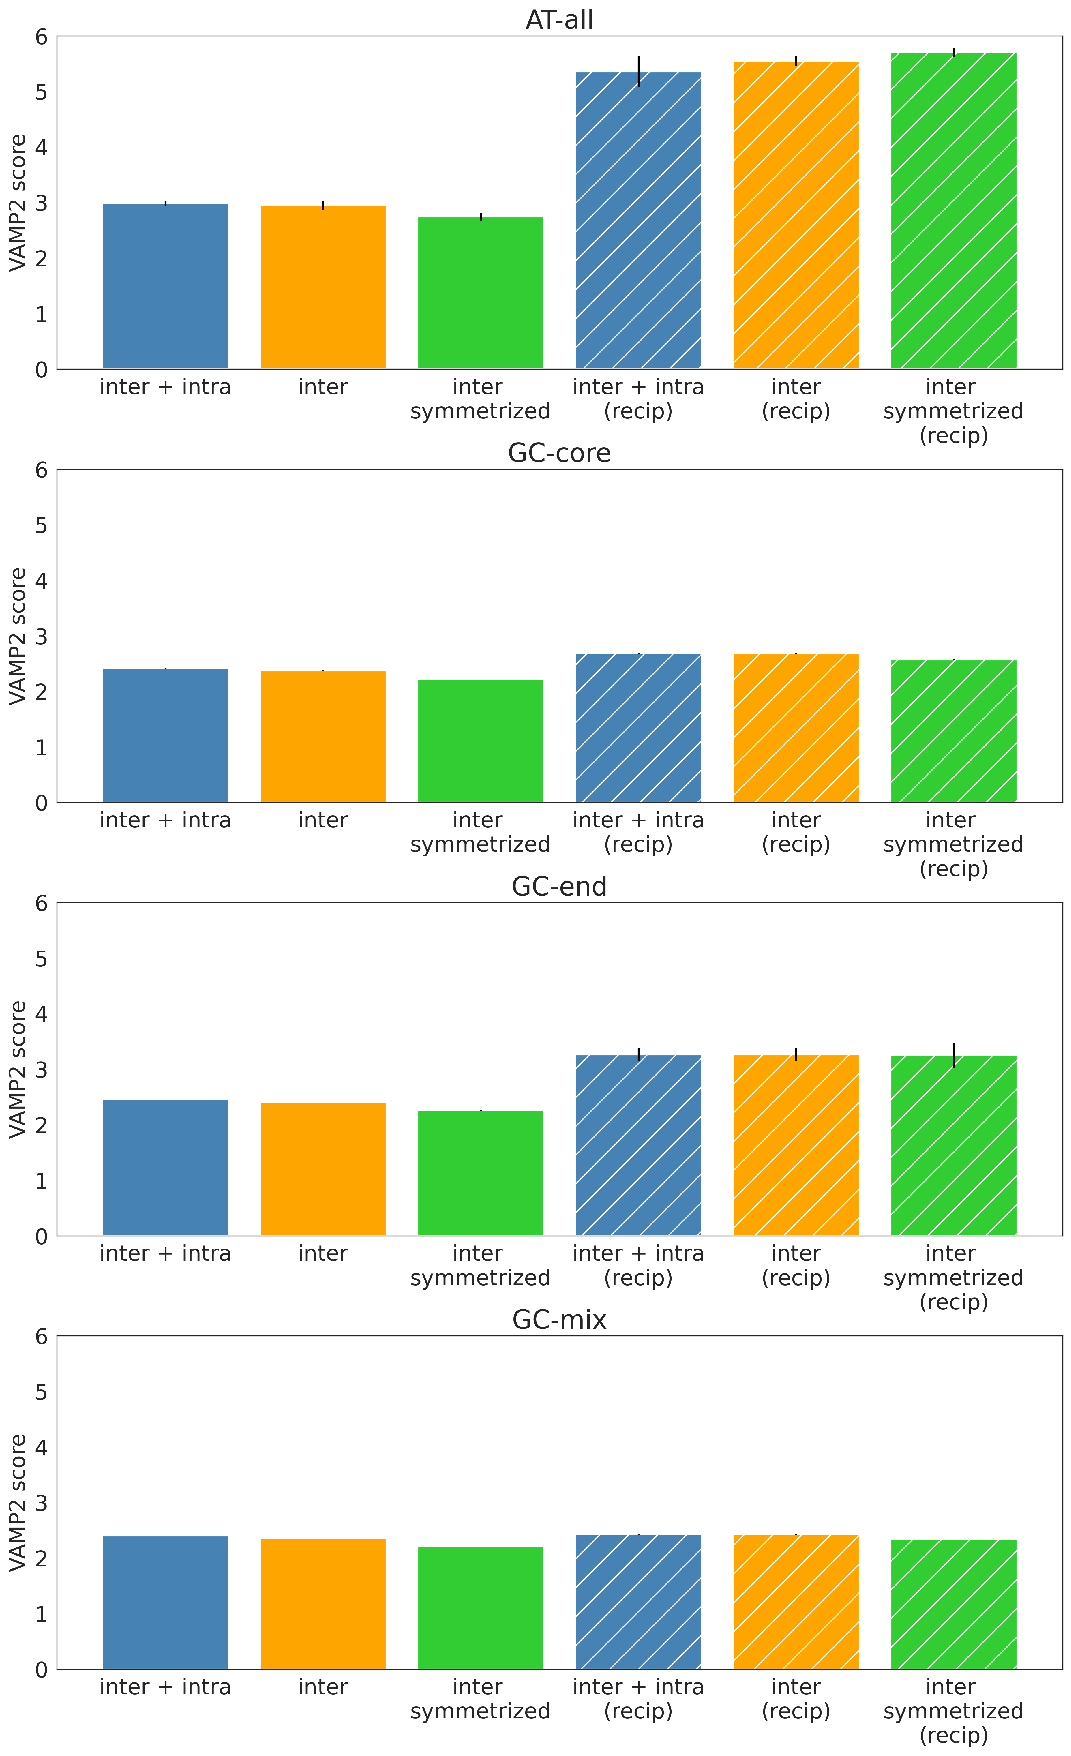
\includegraphics[width=\textwidth]{Fig1.pdf}
        \caption{Experimental measurements and computational predictions of slow and fast at T-jump IR responses. Results are reported in terms of the final T-jump temperature. (a) The experimental and simulated slow rate constants $k_d^\mathrm{slow}$ corresponding to duplex dissociation over long time scales. \rood{We apply a fluctuation correction proposed by Ouldridge et al.\citep{Ouldridge2010ExtractingSimulations} to account for finite-size effects and ensure an asymptotically correct dimer fraction} (b) The experimental and simulated fast rate constant $k_d^\mathrm{fast}$ corresponding to terminal base-pair fraying on short time scales. The simulation results are corrected by a sequence-independent scaling factor that corrects for a 10$\times$ acceleration of the slow dissociation dynamics and 120$\times$ acceleration of the fast fraying dynamics. The simulated temperature in all cases is subjected to a (+4) K corrective calibration to account for an observed systematic under-prediction of the melting temperature by the 3SPN.2 model}
        \label{fig:relaxation-comparison}
	\end{center}
\end{figure}


In Fig.~\ref{fig:relaxation-comparison}a we observe an exponential increase of $k_d^\mathrm{slow}$ with temperature, as expected from the large enthalpic barrier to duplex dissociation.\cite{Craig1971RelaxationOligonucleotides,Porschke1971CooperativeTransition,Williams1989LaserDGCATGC} Under the time and temperature calibration corrections, we see generally very good agreement between the computational and experimental curves. Of the four sequences, GC-core shows the largest discrepancy between computation and experiment, although the general exponential trend is preserved. This may be a result of its high propensity to fray (cf.\ Section \ref{sec:GC-core}). In Fig.~\ref{fig:relaxation-comparison}b we expose a largely linear dependence of $k_d^\mathrm{fast}$ upon temperature for AT-all, GC-end, and GC-mix compared to an exponential dependence for GC-end. These trends can be understood in light of the comparatively larger enthalpic barrier for dissociation of the terminal G:C base pair in GC-end compared to that for the A:T terminal pair in the other three sequences. Again we see good agreement between the scaled computational predictions and the experimental T-jump measurements. The favorable comparison of computation and experiment provides support for the capacity of the 3SPN.2 model to reliably reproduce sequence-dependent trends in the slow and fast kinetics of the four DNA oligomers \rood{, and lends confidence in the use of these data for the parameterization of Markov state models of the long-time dynamics of each sequence. We observe that the dynamical fingerprinting approach presents an elegant means to compare experimental relaxation data directly against a Markov state model extracted from simulation data in terms of a ``fingerprint'' of peaks with amplitudes and time scales related to the relaxation of particular system observables~\citep{Noe2011DynamicalExperiments}. These techniques have been previously employed to in applications to base stacking of DNA dinucleoside monophosphates~\citep{Remington2019MolecularKinetics} and RNA~\citep{Pinamonti2017}. We explored the use of this approach to validate the MD simulation data but encountered challenges in resolving fast dynamical motions below the lag time of the fitted MSM and the extremely high computational cost of collecting sufficient simulation data to fit MSMs at each temperature for which experimental data was collected. Accordingly, we instead elected to perform a direct comparison between the experimental data and MD trajectories to validate the simulations themselves, then proceed to train MSMs over these data and conduct analysis and experimental tests of the MSM predictions.}.






\subsection{SRV-MSMs for each sequence}

We now proceeded to construct Markov state models (MSMs) from 1 ms of aggregated simulation trajectories for each of the four sequences at their respective melting temperatures to generate sequence-dependent kinetic models. MSMs define the long-lived metastable macrostates of the system, their equilibrium occupancies, and the equilibrium transition probabilities between them. As such, they are extremely valuable in providing both a quantitative predictive model and a physically comprehensible mechanistic understanding of the long-time dynamical evolution of the system between an ensemble of metastable macrostates. We present in Fig.~\ref{fig:allseq_table} the inferred MSMs for each of the four 10-base DNA sequences. Across all four sequences we identify a totality of seven metastable macrostates corresponding to the fully hybridized state (H) in which all native base pairings are intact, four shifted states in which the strands are translated out-of-register by two or four bases in the 5$^\prime$ (5S2, 5S4) or 3$^\prime$ (3S2, 3S4) direction, a frayed state (F4) -- unique to GC-core -- in which four terminal A:T base pairs are unbound, and the fully dissociated state (D). We present these seven macrostates in Fig.~\ref{fig:allseq_table}a along with schematic and cartoon renderings of representative microstates contained within each of these macrostates. \rood{The representative microstates emblematic of each macrostate were selected randomly from those possessing high ($>$99\%) macrostate membership probabilities. Since the microstate ensemble exhibits a range of conformations, however, it is useful to characterize the degree of structural heterogeneity to determine the degree to which these microstates are emblematic of the distribution. In Fig.~S{\blauw{X}} we present a projection of our macrostates into two physical order parameters -- the degree of 3$^\prime$ shift and degree of 5$^\prime$ shift -- to provide an interpretable embedding of the macrostates that exposes base pairing patterns and structural heterogeneity within the microstate ensemble. In all cases, we find these microstate distributions to be relatively narrowly focused within the low-free energy core of each macrostate such that a single archetypal microstate is indeed a good representative for the ensemble and an accurate representation of the base pairing pattern of the macrostate.} In Fig.~\ref{fig:allseq_table}b we present the occupancy probabilities of each state at thermodynamic equilibrium. By virtue of the fact that each sequence is simulated at its corresponding melting temperature (T$_\mathrm{m}$), the probability of the dissociated state (D) is, by construction, approximately equal to the sum of the probabilities over the remaining six states (H, 5S2, 3S2, 5S4, 3S4, F\rood{4}). In Fig.~\ref{fig:allseq_table}c we present a visualization of the macrostate MSMs for each of the four sequences showing the connectivity between the identified macrostates. The macrostates are represented as orange circles in proportion to their equilibrium probabilities and the grey arrows indicate the probability of hopping from one macrostate to another under one time step of the kinetic model. The fluxes between the macrostates provide a wealth of high-level, interpretable information on the sequence-dependent metastable states and hybridization/dehybridization pathways. Immediately, we identify that the AT-all sequence possesses a rich and complex dynamical landscape comprising six metastable states whereas at the other end of the spectrum GC-mix exhibits far simpler two-state ``all-or-nothing'' behavior. In Fig.~\ref{fig:allseq_table}d we present the so-called implied time scales of each MSM. These time scales correspond to the relaxation times of the DNA dimer among its constituent metastable macrostates. The leading implied time scale for each system corresponds to the characteristic time scale for hybridization/dehybridization. Since each system is simulated at the same concentration and at its respective melting temperature, it is not surprising that the leading time scale is approximately equal for all four systems and corresponds to the characteristic time scale for hybridization/dehybridization. The spectrum of higher order time scales corresponds to increasingly quicker relaxations between the metastable macrostates within the kinetic model and resolve the interesting sequence-dependent differences in the hybridization/dehybridization kinetic pathways. The total number of implied time scales is typically one fewer than the number of metastable macrostates and the existence of large implied time scales is indicative of slowly relaxing kinetic processes. The dense spectrum of slow implied time scales for AT-all is indicative of its relatively complex kinetic landscape whereas that for the two-state GC-mix comprises only a single time scale corresponding to hybridization/dehybridization. We now proceed to analyze in detail the sequence-dependent thermodynamics, kinetic, and mechanisms exposed by the four MSMs.

\begin{figure}[ht!]
	\begin{center}
        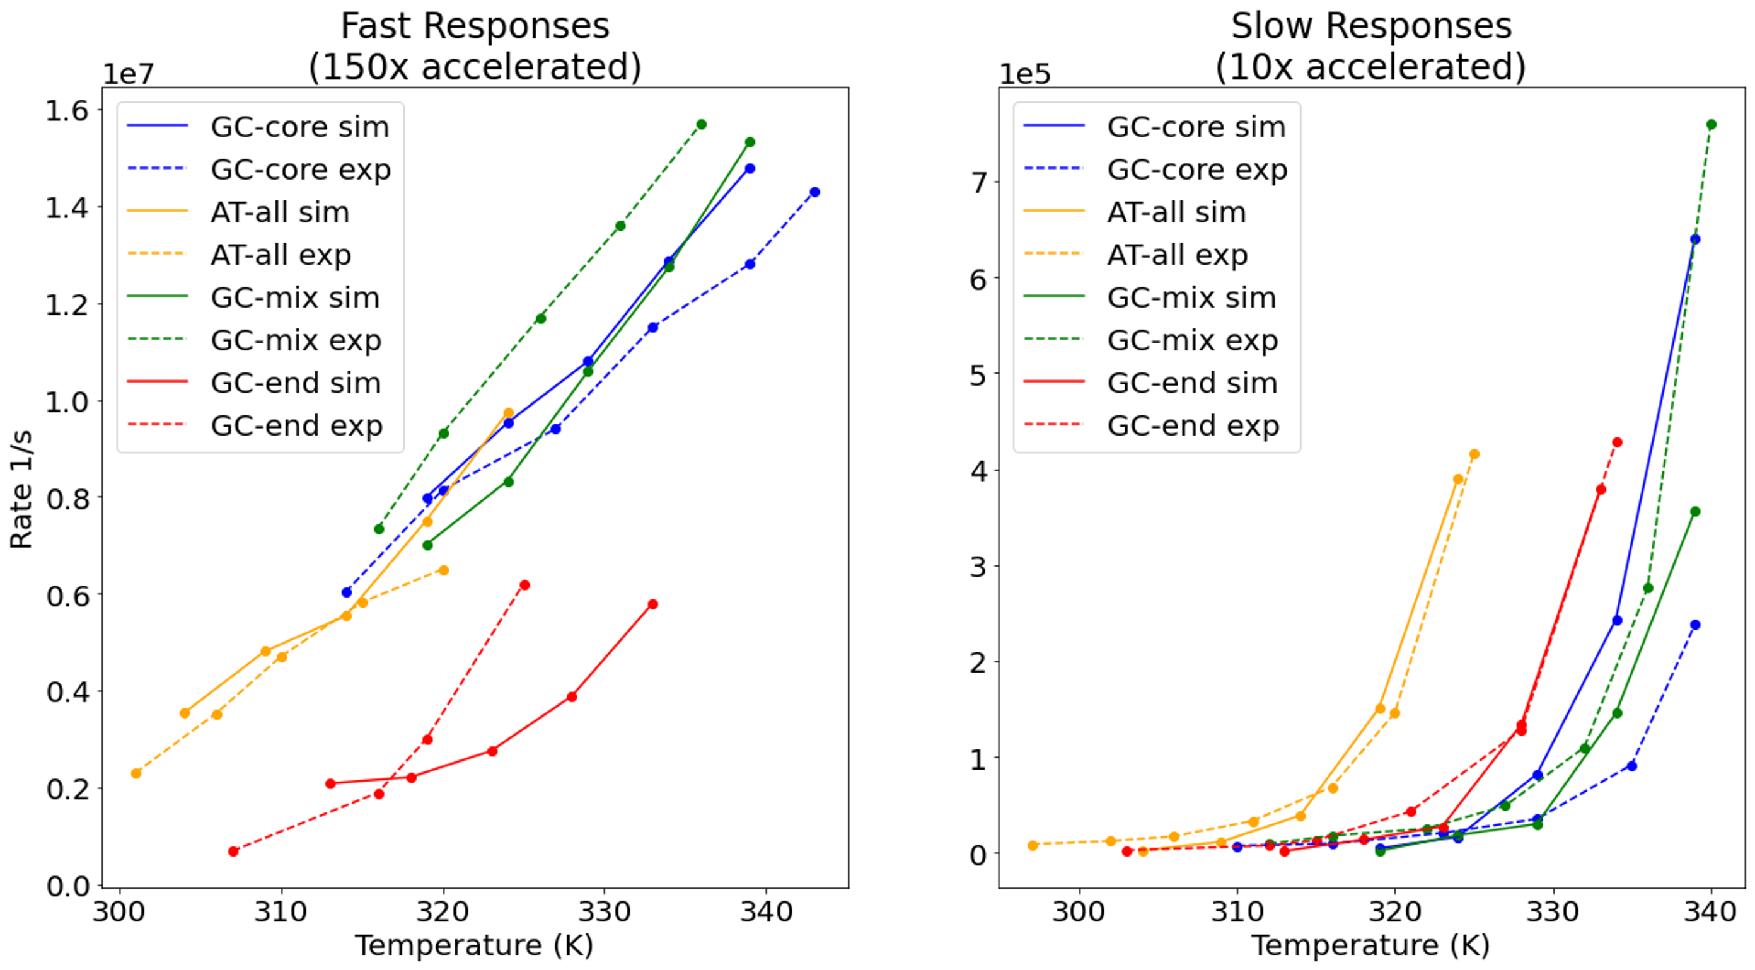
\includegraphics[width=1.0\textwidth]{Fig2.pdf}
	\end{center}
\end{figure}
\begin{figure}[ht!]
        \caption{Thermodynamic and kinetic predictions of the sequence-specific MSMs \rood{fitted at the sequence melting temperatures} for AT-all, GC-end, GC-core, and GC-mix. (a) \textbf{Macrostates.} Schematic representation of the seven metastable macrostates occupied by one or more of the four sequences: fully hybridized state (H), two-base out-of-register shifted states in the 5$^\prime$ (5S2) or 3$^\prime$ (3S2) direction, four-base out-of-register shifted states in the 5$^\prime$ (5S4) or 3$^\prime$ (3S4) direction, and the fully dissociated state (D). The line drawings represent the 10-base self-complementary sequences, where red-to-blue contacts indicates (possible) WC base pairing and black indicates an unbound bases. Adjacent to each line drawing we provide representative molecular structures corresponding to that macrostate. (b) \textbf{Thermodynamics.} Histograms reporting the number of the $10^7$ total frames within the 1 ms of simulation trajectories observed to occupy each of the seven macrostates, corresponding to our numerical estimates of the equilibrium occupancy probabilities. Uncertainties are calculated across 100 MSMs using a Bayesian MSM estimation are reported for each bar and are very small compared to the total counts. \rood{Values are reported on a log y-axis to make the small populations of the shifted and frayed states visible.} (c) \textbf{Kinetic networks.} MSMs illustrating the kinetic network for each sequence. The orange circles correspond to the macrostates occupied by each sequence and are labeled by the macrostate codes reported in panel a. The radii of the circles is proportional to the logarithm of the equilibrium occupancy populations reported in panel b. Molecular renderings of an illustrative snapshot from the coarse-grained molecular simulations are provided next to each macrostate. The grey arrows between macrostates indicate the presence of a probability flux between this pair of states at equilibrium and the arrow thickness is proportional to the flux. (To avoid congesting the diagram, arrows are not reported for probability fluxes lower than $3\times10^{-6}$.) The numerical value overlaid on each arrow reports the conditional probability that a system occupying the macrostate at the start of the arrow at time $t$ will transition to the macrostate at the end of the arrow by time $(t+\tau)$, where $\tau$=1.2 ns is the lag time corresponding to a single time step of the MSM. Large orange circles correspond to thermodynamically favorable states and large grey arrows correspond to kinetically favorable transitions. (d) \textbf{Kinetic time scales.} Distribution of MSM implied time scales for each sequence. The leading implied time scale corresponds to the characteristic time scale for hybridization/dehybridization and is approximately equal for all systems since simulations were conducted at the same concentration and at the respective melting temperatures. The higher order implied time scales correspond to a spectrum of kinetic relaxations between the constituent macrostates in the MSM corresponding to shifted and/or frayed states.
    }
    \label{fig:allseq_table}
\end{figure}





\subsection{Comparison of MSM thermodynamic predictions with NN model} \label{sec:NN}

We first compare the thermodynamic predictions for the equilibrium macrostate probabilities \rood{made by the MSM models fitted at the sequence melting temperatures} to those of the nearest neighbor (NN) model as a popular empirical model of DNA hybridization thermodynamics. The NN model predicts the free energy of duplex formation as a sum over helix initiation terms and the hybridization free energies of nearest neighbor pairs of bases that account for both the specific WC pairings and the modulating effects of the local (i.e., nearest neighbor) environment.~\citep{SantaLucia1998AThermodynamics, Santalucia2004TheMotifs} The parameters of the NN model were estimated by regressing over 108 experimental measurements to furnish a predictive model for the free energy of association as a function of DNA sequence and explicitly account for stacking contributions of native pairs, internal mismatches, and dangling ends. We apply the NN model to predict the free energy $F^\mathrm{NN}$ of each of the macrostates occupied by each of the four sequences. A full accounting of our application of the NN model is provided in the \blauw{Supporting Information}. The free energy of each macrostate is related to its equilibrium occupancy probability $P$ via the statistical mechanical relationship $F = -k_B T \ln P + C$, where $T$ is temperature, $k_B$ is Boltzmann's constant, and $C$ is an additive constant reflecting our ignorance of the absolute scale of free energies. We use this relationship to convert the equilibrium occupancy probabilities predicted by our MSM and reported in Fig.~\ref{fig:allseq_table}b into free energies $F^\mathrm{MSM}$. The unknown additive constants preclude comparisons of absolute free energies between the MSM and NN model, but it is legitimate to compare relative free energies between pairs of macrostates since the additive constant cancels in taking differences. As such, we arbitrarily set the additive constant $C$ in both the MSM and NN model such that the hybridized state H defines a zero free energy reference state and we report the stability of all macrostates relative to the hybridized state as $\Delta F^\mathrm{NN} = F^\mathrm{NN} - F_H^\mathrm{NN}$ for the NN model and $\Delta F^\mathrm{MSM} = F^\mathrm{MSM} - F_H^\mathrm{MSM}$ for the MSM. 

As illustrated in Fig.~\ref{fig:NN_table}, we see that the MSM tends to predict higher free energies for the out-of-register shifted macrostates 5S2, 3S2, 5S4, and 3S4 relative to the H state compared to the NN model. The NN and MSM predictions for the frayed state F4 are in good agreement. Although the shifted state trends are in qualitative agreement, what is the root of the quantitative discrepancy of the MSM and NN models in the predicted relative stabilities? First, the MSM is constructed bottom-up from molecularly detailed 3SPN.2 simulations whereas the NN model is fitted top-down by regression against experimental data. There are approximations inherent in the 3SPN.2 model, not least of which is the coarse-grained representation that integrates over atomic degrees of freedom, and in the NN model that was fitted to limited experimental data assuming a low-order expansion in terms of nearest neighbor additive contributions. Second, although 3SPN.2 is expected to capture some dangling end stabilization effects through base stacking and cross-stacking interactions, the model was not parameterized to fully capture the enthalpic contributions of the interaction of unbound bases with terminal base pairs, whereas this term is explicitly included within the NN model. Third, a well known deficiency of the NN model is the absence of any treatment of inert tails -- free bases that extend beyond the dangling end tend to destabilize the duplex.\citep{DiMichele2014EffectHybridization}

\begin{figure}[ht!]
	\begin{center} 
        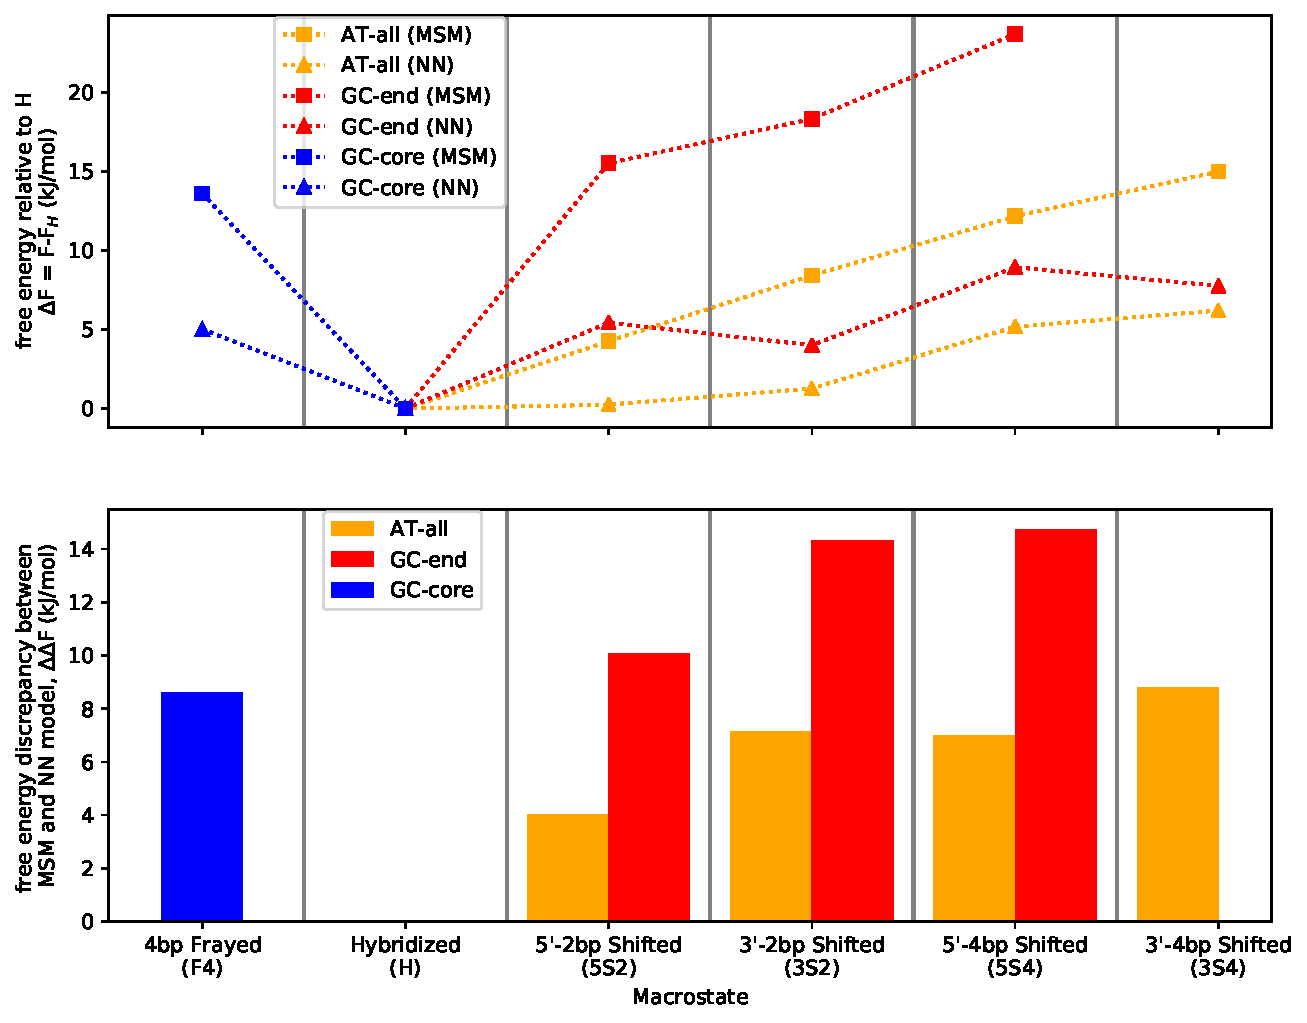
\includegraphics[width=160mm, scale=1]{Fig3.pdf}
        \caption{Comparison of the macrostate free energy predictions of the MSMs and nearest neighbor (NN) thermodynamic model \rood{at the sequence melting temperatures}.~\citep{SantaLucia1998AThermodynamics, Santalucia2004TheMotifs} (a) Free energies of each macrostate relative to the hybridized state $\Delta F = F - F_H$. We define the hybridized state H to possess a free energy of zero and take care to only compare relative free energies (i.e., $\Delta F$) between the MSM and NN model. (b) Discrepancy between the macrostate relative free energy predictions $\Delta \Delta F = \Delta F^\mathrm{MSM} - \Delta F^\mathrm{NN}$ of the MSM relative to the NN model. The MSM tends to predict higher relative free energies (i.e., lower occupancy probabilities) for the out-of-register shifted states 5S2, 3S2, 5S4, 3S4 relative to the hybridized state H compared to the NN model.}
        \label{fig:NN_table}
	\end{center}
\end{figure}

We can further explore the role of inert tails upon macrostate stability by analyzing the AT-all and GC-end sequences that occupy out-of-register shifted macrostates 5S2 and 3S2 comprising a one-base inert tail and 5S4 and 3S4 comprising a three-base inert tail (cf.\ Fig.~\ref{fig:allseq_table}a). For both sequences, our simulations show that 5S2 is both the most stable of shifted states relative to H (Fig.~\ref{fig:NN_table}a) and has the smallest discrepancy ($\sim$4 kJ/mol AT-all, $\sim$10 kJ/mol GC-end) compared to NN predictions (Fig.~\ref{fig:NN_table}b). The 3S2 and and 5S4 states have nearly the same deviation from NN predictions ($\sim$7 kJ/mol AT-all, $\sim$15 kJ/mol GC-end), indicating that longer tails in the 5$^\prime$ direction are as destabilizing as shorter tails in the 3$^\prime$ direction. It is known from differential scanning calorimetry studies~\citep{Dickman2012ThermodynamicDNAs} that 3$^\prime$ inert tails are more destabilizing than 5$^\prime$ tails, with the differential behavior attributed to a combination of 5$^\prime$ tails preferentially stacking on the core duplex and 3$^\prime$ tails perturbing the duplex structure. \citep{Doktycz1990ThermodynamicC, Dickman2012ThermodynamicDNAs, DiMichele2014EffectHybridization}. Both the NN and MSM predictions for AT-all are consistent with this trend (i.e., $F_\mathrm{3S2} > F_\mathrm{5S2}$ and $F_\mathrm{3S4} > F_\mathrm{5S4}$). For GC-end, the MSM and NN models both predict the out-of-register shifted states to be less stable relative to the hybridized state than the corresponding predictions for AT-all. This is in line with expectations since the terminal G:C pairs in GC-end decrease by two the number of available WC pairings in out-of-register shifted states compared to AT-all. The GC-end NN predictions run contrary to the expectation that the 3$^\prime$ inert tails should be more destabilizing than the 5$^\prime$ tails, whereas the MSM predictions are consistent with this trend. Indeed, the MSM model for GC-end does not identify the 3S4 macrostate as a stable metastable conformation for the duplex.

In sum, the qualitative trends in the macrostate thermodynamic stabilities are in good agreement between the MSM and NN models, but show quantitative discrepancies for macrostates possessing inert tails. In these instances the MSM predicts these macrostates to be less stable relative to the hybridized state compared to the NN model predictions by 4.0-14.5 kJ/mol. The MSM predictions are also consistent with the experimental expectation that 3$^\prime$ inert tails should be more destabilizing than the 5$^\prime$ tails, whereas the NN predictions can be in conflict with this trend.





\subsection{Out-of-register states facilitate hybridization and dissociation dynamics (AT-all, GC-end)}

In addition to thermodynamic stabilities, the macrostate MSM also furnishes quantitative and interpretable predictions of hybridization and dehybridization pathways and mechanisms \rood{at the sequence melting temperatures}. \rood{It should be noted that because we are using a reversible MSM framework, detailed balance is enforced by construction.} We now proceed to analyze these predictions for each of the four sequences and illuminate the relationship between sequence and dynamics. Two of our sequences, AT-all and GC-end, support out-of-register metastable states, and we commence our analysis with the role of these shifted states.

AT-all possesses the richest and most complex MSM of the four sequences by virtue of its repetitive nature, comprising a hybridized state (H), dissociated state (D), and four out-of-register shifted states (5S2, 3S2, 5S4, 3S4) (Fig.~\ref{fig:allseq_table}c). Analysis of the MSM transition probabilities reveal a critical role of the shifted states in mediating hybridization and dehybridization. Commencing from the dissociated state D, we observe approximately equal probabilities for transitions to each of the other five states, such that a transition to one of the out-of-register shifted states 5S2, 3S2, 5S4, or 3S4 is approximately 2.2 times more likely than a direct transition to the hybridized state H. Commencing from the hybridized state H, however, a direct transition to the dissociated state is approximately 1.2 times more likely than a transition to one of the two-base shifted states 5S2 or 3S2. Once in one of the four shifted states, the 5$^\prime$ vs.\ 3$^\prime$ overhang and degree of shifting play an important role in determining whether the duplex will transition to more shifted states, more aligned states, or completely dissociate. Transitions from more shifted states towards more aligned states (i.e., 5S4 $\rightarrow$ 5S2, 5S2 $\rightarrow$ H, 3S4 $\rightarrow$ 3S2, 3S2 $\rightarrow$ H) are approximately an order of magnitude more probable than the reverse transitions from more aligned states to more shifted states. The largest single transition probability from the four shifted states 5S2, 3S2, 5S4, and 3S4 is, however, back to the dissociated state D. Consistent with the higher destabilizing effect of 3$^\prime$ inert tails relative to 5$^\prime$ tails,~\citep{Doktycz1990ThermodynamicC, Dickman2012ThermodynamicDNAs, DiMichele2014EffectHybridization} the 3S4 $\rightarrow$ D transition probability is twice as large as the 5S4 $\rightarrow$ D, and the 3S2 $\rightarrow$ D is four times larger than the 5S2 $\rightarrow$ D. The transition probability from the 5S2 and 3S2 states back to the dissociated state D is equal to or greater than the transition probability to the hybridized state. A transition path theory analysis of the MSM reveals that 33\% of productive hybridization trajectories D $\dashrightarrow$ H (where the dashed arrow indicates the combination of both direct and indirect pathways) and dehybridization trajectories H $\dashrightarrow$ D proceed through one or more out-of-register shifted states. Among these out-of-register hybridization pathways, the D $\dashrightarrow$ 5S2 $\dashrightarrow$ H transition is predicted to occur 57\% of the time. A mean first passage time (MFPT) analysis returns a MFPT for D $\dashrightarrow$ H of 3.0 $\mu$s and for H $\dashrightarrow$ D of 2.5 $\mu$s. As expected by the fact that the calculations are performed at the melting temperature, the MFPTs are approximately equal.  

GC-end comprises the next most complex MSM. The introduction of the G:C pairs at the termini of the strands maximally preserves the repetitive tract of A:T base pairings such that the GC-end MSM possesses all of the same macrostates in its dynamical landscape with the exception of the 3S4 state (Fig.~\ref{fig:allseq_table}c). As discussed in Section \ref{sec:NN}, the 3S4 state is rendered unstable within the lag time of our MSM due to the presence of the destabilizing 3$^\prime$ inert tail and only four WC base pairings compared to six in the case of AT-all. Analysis of the transition probabilities reveal significant differences compared to those in the AT-all kinetic network. Commencing from the dissociated state D, we observe a similar transition probability to the 5S4 state as for AT-all, but once in the 5S4 state there are no significant transition probabilities to any other state except back to D. As such, the 5S4 state acts as a kinetic trap rather than as an intermediate to hybridization. The D $\rightarrow$ H and H $\rightarrow$ D transition probabilities are commensurate with those for AT-all. However, the D $\rightarrow$ 5S2 and D $\rightarrow$ 3S2 transition probabilities are half or less of those in AT-all, and the reverse transitions are an order of magnitude larger. This may be attributed to the reduced thermodynamic stability of the 5S2 and 3S2 states in GC-end that comprise only six WC pairs compared to eight in AT-all (cf.\ Fig.~\ref{fig:NN_table}). The 5S2 $\rightarrow$ H and 3S2 $\rightarrow$ H transition probabilities are more than an order of magnitude larger than in AT-all, which may again be attributed to the lower thermodynamic stability of the two shifted states relative to the hybridized state H. Again, the transition probabilities out of the 3S2 state to D or H are comparatively higher than those out of the 5S2 state, consistent with the increased destabilizing effect of 3$^\prime$ inert tails.~\citep{Doktycz1990ThermodynamicC, Dickman2012ThermodynamicDNAs, DiMichele2014EffectHybridization} Commencing from the hybridized state H, a direct transition to the dissociated state is approximately seven times more likely than a transition to one of the two-base shifted states 5S2 or 3S2. A transition path theory analysis of the MSM reveals that only 7\% of hybridization events D $\dashrightarrow$ H and dehybridization events H $\dashrightarrow$ D proceed through one or more out-of-register shifted states. The significantly reduced role for out-of-register shifted states in mediating the hybridization and dissociation pathways for GC-end relative to AT-all is consistent with the reduced thermodynamic stability of these states due to the elimination of possible out-of-register WC base pairing for the terminal G:C pairs and therefore a reduced accessibility of these states in the GC-end kinetic network. We compute a MFPT for D $\dashrightarrow$ H of 1.6 $\mu$s and for H $\dashrightarrow$ D of 2.1 $\mu$s, which are again approximately equal.

The out-of-register kinetic landscape that defines AT-all and GC-end hybridization have been explored by a number of previous computational studies. Simulations have identified internal displacement mechanisms capable of correcting base pair alignment in 3SPN.2 \citep{Hinckley2014Coarse-grainedEffects} as well as in the coarse-grained oxDNA \citep{Romano2013DNADependence} and BioModi \citep{Markegard2015} models. In all cases, these mechanisms were shown to be crucial components of the hybridization pathway for homogeneous and repetitive sequences. Xiao et al.\ performed an all-atom energy landscape-based analysis of 5$^\prime$-GGGGGG-3$^\prime$ and 5$^\prime$-GCGCGC-3$^\prime$ hexamers.~\citep{Xiao2019} Out-of-register states for 5$^\prime$-GCGCGC-3$^\prime$ hexamers were identified as deep kinetic traps along the hybridization pathway and ``slithering'' through these states did not provide a significant hybridization pathway compared to an alternative ``zippering'' mechanism. (In contrast, slithering through out-of-register shifted states and zippering served as two parallel pathways for hybridization of 5$^\prime$-GGGGGG-3$^\prime$.) This stands in contrast to our results for our AT-all (5$^\prime$-ATATATATAT-3$^\prime$) sequence, in which out-of-register states participated in 33\% of productive hybridization events. It is conceivable that the stronger hydrogen bonding in G:C WC pairs relative to A:T pairs may render out-of-register shifted states less favorable to hybridization by suppressing fluctuation-driven rearrangements,~\citep{Yakovchuk2006Base-stackingHelix,Zacharias2020Base-PairingFormation} but additional studies would be required to reconcile these observations.





\subsection{Central GC placement induces long-lived frayed states (GC-core)} \label{sec:GC-core}

The GC-core MSM represents a departure from the relatively rich and complex kinetic networks dominated by out-of-register shifted states to a much simpler one dominated by fraying (Fig.~\ref{fig:allseq_table}c). The MSM contains only three states -- hybridized H, dehybridized D, and frayed F4. The F4 state is unique to GC-core and contains up to six WC pairs -- the two central G:C core pairs and as many as four A:T pairs on one side or other of the core, while the other run of four A:T pairs remains free. (As expected by symmetry, the particular AT run that is free occurs with equal probability on either side of the core.) Although partially frayed states containing less than four free A:T bases on either end of the duplex are common, these tend to interconvert faster than the lag time and are not registered as metastable within our MSM. Our model reveals the absence of any direct hybridization or dehybridization transitions between the H and D states, with all pathways passing through the frayed state F4. Previous studies would suggest that hybridization of this sequence should proceed via a zippering mechanism, wherein upon formation of the strong central G:C WC base pairings the duplex helix should rapidly assemble in a middle-out fashion.~\citep{Romano2013DNADependence, Yin2011KineticsHybridization} Our results are partially consistent with this expectation, but reveal the frayed state F4 to be unexpectedly metastable, serving as a long-lived state with an mean life time of 1.8 ns. The stability of the state is attributable to the enthalpic stabilization offered by the up to six WC pairs and the entropic stabilization associated with the configurational entropy of the two free AT-tails.

Analysis of the transition probabilities show that commencing from the F4 state, progression to the hybridized state F4 $\rightarrow$ H is 25 times more likely than dissociation F4 $\rightarrow$ D. Thus once a D $\rightarrow$ F4 transition has occurred, a F4 $\rightarrow$ H transition will likely proceed; concomitantly, H $\rightarrow$ F4 events tend to fall back to the H state and are less likely to proceed to complete dissociation D. We noted in Section \ref{sec:time} that fraying dynamics in the 3SPN.2 model appear to be significantly accelerated relative to center-of-mass translation, and it is conceivable that this may lead to elevated sampling of the F4 state within the computational model relative to experiment and the induction of more frequent dissociation. Moreover, since GC-core is the sequence most prone to fraying, this effect could be the root of the relatively poorer agreement of the $k_d^\mathrm{slow}$ response for GC-core compared to the other sequences due to an artificially elevated computational prediction of this rate (Fig.~\ref{fig:relaxation-comparison}a). Our model predicts a MFPT for D $\rightarrow$ F4 $\rightarrow$ H of 3.4 $\mu$s and for H $\rightarrow$ F4 $\rightarrow$ D of 2.9 $\mu$s, which are again approximately equal.

Lattice models have previously identified frayed states as putative intermediates in DNA hybridization/dehybridization.\citep{Araque2016LatticeCooperativity, Phys2019,Sanstead2016} Araque et al.\ studied a 5$^\prime$-ATGCGCAT-3$^\prime$ octomer using a lattice model and identified a symmetrically A:T frayed state as a crucial part of the duplex transition path.\citep{Araque2016LatticeCooperativity} We previously studied the four sequences that are the subject of the present work using T-jump IR and 2D IR spectroscopy and identified GC-core as possessing the highest deviation from two-state behavior during dissociation when neglecting out-of-register contributions.\citep{Sanstead2016} This result was interpreted to arise from loss of A:T contacts and fraying around the central G:C core, and this hypothesis was supported by lattice model calculations that predicted the GC-core conformational ensemble to possess substantially more frayed configurations than the other three sequences.~\citep{Phys2019} Follow-up T-jump measurements and Smoluchowski simulations on model 1D free energy landscapes showed that AT termini fraying was an effectively barrierless process characterized by rapid inter-conversion between all accessible frayed states.\citep{Sanstead2018DirectDehybridization} These prior results are consistent with the present findings that expose the GC-core sequence to be the only sequence that occupies the F4 frayed state and therefore the only one possessing a metastable frayed state on time scales exceeding the $\tau$=1.2 ns lag time of our MSMs.





\subsection{Disruption of repetitive AT tracts promotes two-state ``all-or-nothing'' kinetics (GC-mix)}

The GC-mix sequence is the only one of the four sequences studied that exhibits simple two-state ``all-or-nothing'' behavior.~\citep{Xiao2019, Araque2016LatticeCooperativity, Sikora2013ModelingIntermediates, Sanstead2016} \rood{This characterization is intended to reflect that the mechanistic observation that} GC-mix MSM comprises just two states, the hybridized H and dehybridized D (Fig.~\ref{fig:allseq_table}c), indicating that association and dissociation of the strands proceeds directly without passing through any metastable intermediate states resolvable under the $\tau$=1.2 ns lag time of our MSM. \rood{Indeed, the sequence's propensity to fray in simulation and the role of termini fraying in dissociation experiments \citep{Sanstead2016} indicate that there remain deviations from ``all-or-nothing'' behavior which are not fully captured within the MSM lag time. (We note that ``all-or-nothing'' can also be used, somewhat ambiguously, to refer to a two-state thermodynamic model where the hybridized and dehybridized are separated by a large free energy barrier but that the transitions between them may proceed through a network of metastable states.)} The two-state behavior appears to arise as a consequence of the placement of the G:C pair that maximally disrupts the repetitive AT tract within the decamer and destabilizing either out-of-register shifted states or frayed states. We note that we do observe substantial transient fraying of the terminal two-base AT tails within our dynamical simulations, but these frayed states are not sufficiently thermodynamically stable to produce a metastable macrostate within the resulting MSM. This stands in contrast to the metastable F4 state populated by GC-core. Our MSM predicts a MFPT for D $\rightarrow$ H of 2.9 $\mu$s and for H $\rightarrow$ D of 2.3 $\mu$s, which are again nearly equal.

Given the very simple two-state ``all-or-nothing'' behavior of GC-mix and the absence of any intermediate metastable states, we sought to interrogate our simulation trajectory data to elucidate the hybridization and dehybridization mechanisms. To do so, we followed all 10 intermolecular distances between native WC base pairs and tracked their evolution through a number of hybridization and dehybridization events. We present one representative example of each event in Fig.~\ref{fig:GC-mix_transitions} and four more in \blauw{Fig.~S5}. During the hybridization process, we observe a global decrease in all 10 distances as the strands approach one another and the formation of key native WC contacts immediately prior to duplex formation: specifically, one of the G:C WC pairs and at least one neighboring A:T pair or 2-3 central A:T pairs. This behavior is consistent with a ``nucleation-zippering'' mechanism as has been reported in previous studies.\citep{Wetmur1968KineticsDNA, Porschke1971CooperativeTransition, Sambriski2009SequencePathways,  Yin2011KineticsHybridization} In dehybridization, we observe fraying \rood{of one half of the duplex with the strands remaining associated until the loss of the final A:T pairs and ultimately the last G:C pair}. Qualitatively, we observed some short-lived states composed of two to four native WC base pair contacts immediately before full dissociation occurs, but, in contrast to the F4 state we observe in GC-core, these conformations do not constitute a metastable state within our MSM nor do they tend to reform intact duplexes. These dissociation dynamics are consistent with a ``fraying-peeling'' dehybridization mechanism.\citep{Wong2008TheSimulations, Perez2010Real-timeUnfolding, Zgarbova2014BaseRNA} \rood{We observe that the principle of microscopic reversibility for a molecular system at thermodynamic equilibrium imposes the conditions of detailed balance and symmetry of the classical equations of motion under time reversibility \noter{Add ref: 10.1021/bi800118b}. A consequence of these considerations is that if our system is indeed at equilibrium, then the ``fraying-peeling'' dehybridization mechanism can be considered a reversal of the ``nucleation-zippering'' hybridization pathway since the time-reversed simulation trajectories represent an equally valid sampling of the system dynamics. This is indeed borne out by our mechanistic observations for GC-mix wherein the early stages of ``nucleation-zippering'' proceed by the formation of one G:C contact followed by one or more additional A:T pairs and the late stages by the formation of all remaining WC pairs, which we compare with the early stages ``fraying-peeling'' wherein one half of the duplex frays and the late stages wherein dissociation finally completes by the dissolution of the last few A:T contacts and the final G:C pair.}

\begin{figure}[ht!]
	\begin{center}
	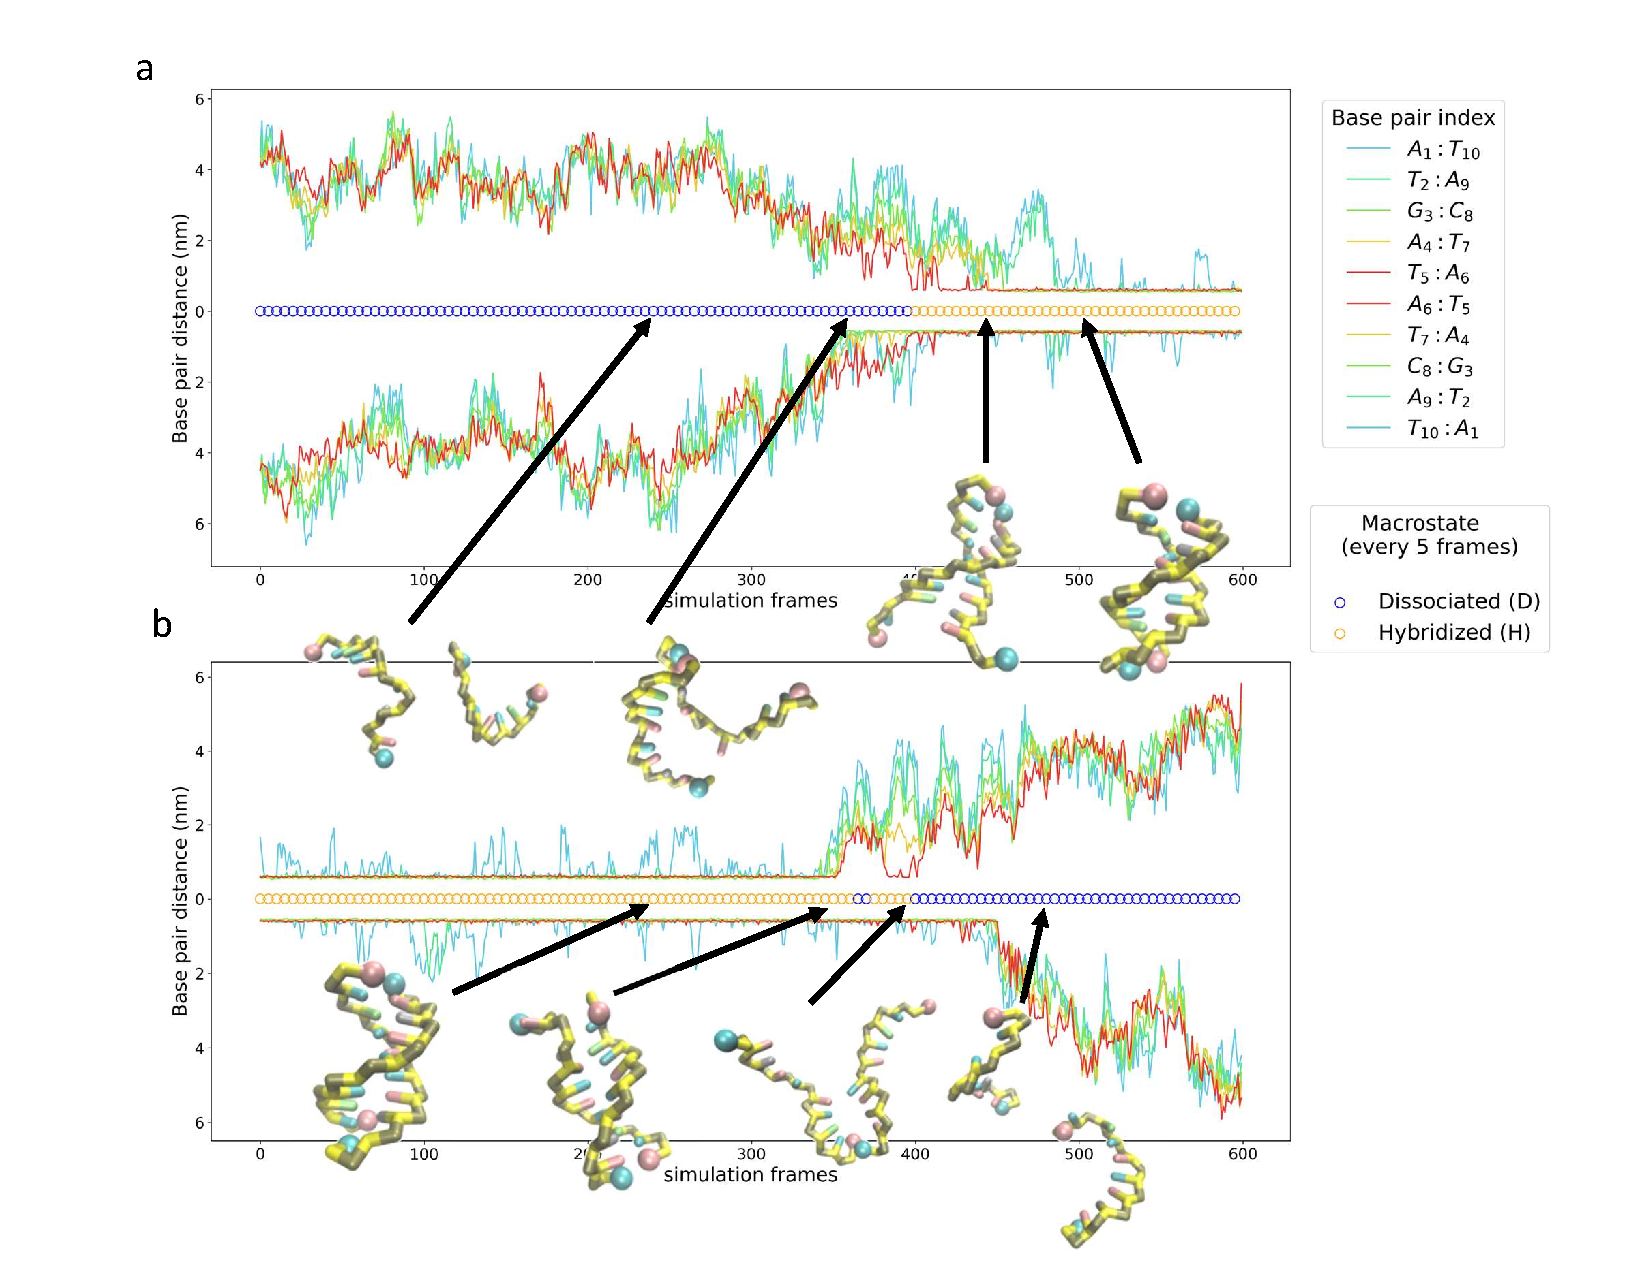
\includegraphics[width=180mm, scale=1]{Fig4.pdf}
        \caption{GC-mix hybridizes by nucleation-zippering and dehybridizes by fraying-peeling. Tracking of the 10 intermolecular distances between native WC base pairs over the course of an (a) hybridization event and (b) dehybridization event. Symmetrically permutable distances (e.g., A$_1$:T$_{10}$ and T$_{10}$:A$_1$) are reflected across the x-axis to avoid congestion in the plot. Circles superposed on the x-axis indicate the instantaneous MSM state assignment as dissociated D (blue) or hybridized H (orange). Hybridization tends to occur by a nucleation-zippering mechanism, wherein a native G:C pair and adjacent A:T pair or 2-3 central A:T pairs first form prior to rapid formation of the duplex. Dehybridization tends to occur by a fraying-peeling mechanism wherein fraying of the two-base AT-tails on one or both sides of the duplex precedes dissociation of the central native base pairs and complete dissolution of the duplex. Four additional hybridization events and four additional dehybridization events are presented in \blauw{Fig.~S5}.
        }
        \label{fig:GC-mix_transitions}
	\end{center}
\end{figure}





\subsection{\label{sec:stretch_comparison}Long-lived metastable shifted states predicted by the MSM are resolved by T-jump IR}

Finally, we sought to validate the predictions of our sequence-dependent MSMs against experimental T-jump IR spectroscopy. T-jump IR measurements commence from a low temperature, apply a step jump in temperature, and track the relaxation of the system to the dehybridized state. We hypothesized that the influence of the out-of-register shifted states present in the AT-all and GC-end sequences upon the system relaxation kinetics should be manifest in the slow and/or fast responses measured by T-jump IR. As discussed in Section \ref{sec:time}, the slow IR response is largely attributed to dissociation events and the fast to terminal base fraying. With regards to the slow response, our MFPT analyses of our MSMs predict out-of-register shifting events (i.e., H $\rightarrow$ 3S2, 5S2, 3S4, 5S4) to proceed on microsecond time scales, which are commensurate with the 1.4 - 2.9 $\mu$s time scales for dehybridization (i.e., H $\rightarrow$ D) for each of the four sequences. As such, we anticipate that the dynamical relaxations associated with out-of-register shifted states proceed on similar time scales to, and may not be distinguishable from, the relaxation to the dehybridized state. Nevertheless, the presence of these out-of-register shifted states in the low-temperature equilibrium ensemble prior to the T-jump step may be observable via their influence on the fast T-jump IR response attributable to fraying. Specifically, we hypothesize that the dangling ends and inert tails present in the out-of-register shifted states should promote an \rood{elevated fraying response over the course of the relaxation that is distinct from that of in-register fraying. This heterogeneity of configurations should lead to heterogeneous dynamics, manifested in the observation of a more stretched relaxation over experimental time scales of 70-100 ns.} Analysis of the MSM equilibrium distributions (Fig.~\ref{fig:allseq_table}b) reveals 10.0\% of the equilibrium ensemble to reside in out-of-register shifted states 3S2, 5S2, 3S4, and 5S4 for AT-all, compared to just 0.23\% for GC-end, and 0\% for GC-core and GC-mix. It is our conjecture that a substantial population of out-of-register shifted states in the pre-T-jump AT-all ensemble should be distinguishable from the GC-end, GC-core, and GC-mix as an elongation of the fast relaxation response associated with terminal base fraying.


We present in Fig.~\ref{fig:T-jump_stretching} our T-jump IR t-HDVE difference spectra and corresponding normalized time traces at 1600 cm$^{-1}$ and 1660 cm$^{-1}$. The signal at 1600 cm$^{-1}$ corresponds to changes in A and T ring vibrations while the signal at 1660 cm$^{-1}$ contains contributions from G and T carbonyl vibrations. Each time trace was fitted to the sum of a stretched exponential and two exponentials $S(t) = A\exp{(-(t/\tau_{\mathrm{fast}})^{\beta_\mathrm{fast}})} + B\exp{(-t/\tau_{\mathrm{slow}})}+C\exp{(-t/\tau_{\mathrm{cool}})}$. The stretched exponential describes the relaxation process from 5 ns to 1 $\mu$s, and the two exponentials describe the signal increase from 1-320 $\mu$s and signal decay from re-hybridization induced by thermal relaxation back to the initial temperature. The fitting parameters $A$, $B$, and $C$ correspond to the relative amplitudes of the three kinetic responses and the stretch factor $\beta_\mathrm{fast}$ to the heterogeneity of fraying dynamics at the fast timescale. A testable prediction of our hypothesis is that the long-lived out-of-register shifted states in AT-all should result in a significantly smaller value for the fitted $\beta_\mathrm{fast}$ parameter (i.e., a more stretched response) relative to those for GC-end, GC-core, and GC-mix. This hypothesis was supported by the experimental time series at both 1600 cm$^{-1}$, where $\beta_\mathrm{fast}^\mathrm{AT-all}$ = 0.3 compared to $\beta_\mathrm{fast}^\mathrm{GC-end}$ = 0.6, $\beta_\mathrm{fast}^\mathrm{GC-core}$ = 0.7, and $\beta_\mathrm{fast}^\mathrm{GC-mix}$ = 0.6, and 1660 cm$^{-1}$, where $\beta_\mathrm{fast}^\mathrm{AT-all}$ = 0.4 compared to $\beta_\mathrm{fast}^\mathrm{GC-end}$ = 0.7, $\beta_\mathrm{fast}^\mathrm{GC-core}$ = 0.6, and $\beta_\mathrm{fast}^\mathrm{GC-mix}$ = 0.6. This result supports our hypothesis and validates a testable prediction of our sequence-dependent MSMs.  

\begin{figure}[ht!]
	\begin{center} 
        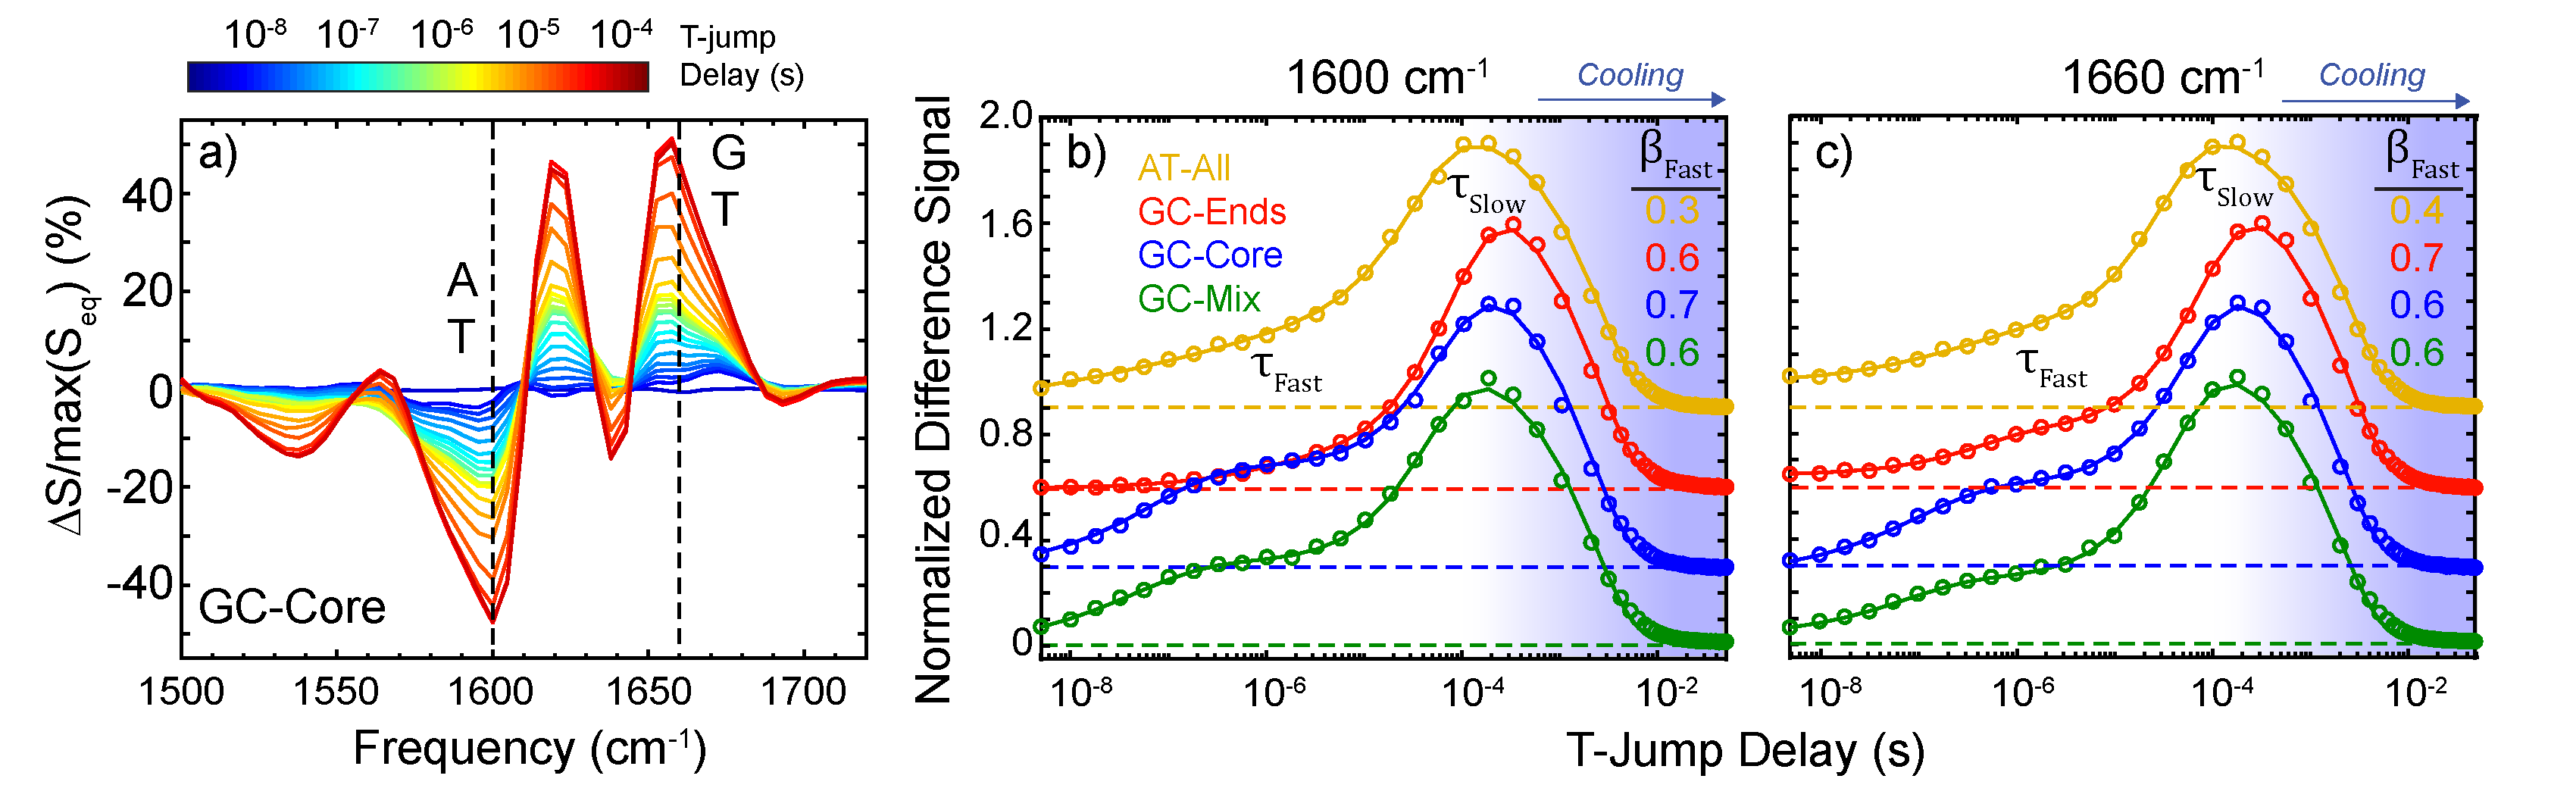
\includegraphics[width=1.0\textwidth]{Fig5.pdf}
        \caption{T-Jump IR responses reflect sequence-dependent conformational heterogeneity. (a) MSM predictions of equilibrium macrostate life times at the sequence melting temperature. (b) Mid-IR t-HDVE difference spectra for GC-core at time delays from 5 ns to 560 $\mu$s. Normalized time traces for each sequence are shown at (c) 1600 cm$^{-1}$ and (d) 1660 cm$^{-1}$. The signal at 1600 cm$^{-1}$ corresponds to changes in A and T ring vibrations while the signal at 1660 cm$^{-1}$ contains contributions from G and T carbonyl vibrations. Each time trace is fit to the sum of stretched exponential with two exponentials (solid lines): $S(t) = A\exp{(-(t/\tau_{\mathrm{fast}})^{\beta_\mathrm{fast}})} + B\exp{(-t/\tau_{\mathrm{slow}})}+C\exp{(-t/\tau_{\mathrm{cool}})}$. The stretched exponential describes the process from 5 ns to 1 $\mu$s, and the two exponentials describe the signal increase from 1-320 $\mu$s and signal decay from re-hybridization induced by thermal relaxation back to the initial temperature. The stretch factor $\beta_\mathrm{fast}$ for the fits at 1600 cm$^{-1}$ and 1660 cm$^{-1}$ are reported directly on the plots in panels c and d.
        }
        \label{fig:T-jump_stretching}
	\end{center}
\end{figure}

   
 
   


\section{\label{sec:conc}Conclusions}

We have conducted an integrated computational and experimental study of the sequence-dependent kinetic mechanisms for the hybridization and dehybridization dynamics of a family of four self-complementary 10-mer DNA oligomers: ATATATATAT (AT-all), GATATATATC (GC-end), ATATGCATAT (GC-core), and ATGATATCAT (GC-mix). We conducted 1 ms of unbiased coarse-grained molecular dynamics simulations \rood{at the melting temperature of each sequence} and employed deep learning techniques to construct high-resolution Markov state models as predictive and interpretable models of the sequence dependent dynamics. T-jump IR spectroscopy was used to calibrate the kinetic time scales of the coarse-grained molecular model and validate the kinetic prediction of the Markov state models that the AT-all sequence should possess long-lived out-of-register shifted states that are detectable within T-jump IR t-HDVE time traces. Our results reveal that the specific placement of interrupting G:C pairs within an otherwise repetitive AT sequence can have a profound impact on the kinetic pathways and mechanisms for association and dissociation of the DNA duplex. In particular, we found AT-all to possess the richest and most complex kinetic landscape of the four sequences that is dominated by out-of-register shifted states that participate in 33\% of complete hybridization events -- pathways leading from the dissociated state to full duplex formation -- and dehybridization events -- pathways from the complete duplex to full dissociation. Introduction of the G:C pairs at the end of the strand maintains an eight-base pair repetitive AT tract and the GC-end kinetic landscape possess all but one of the same out-of-register shifted states as AT-all. Destabilization of the GC-end shifted states relative to AT-all, however, results in a far more limited participation of these states with only 7\% of GC-end hybridization and dehybridization events passing through one or more shifted states. Placing the G:C pairs in the center of the strand maintains two four-base AT tracts either side of the core and results in qualitatively different kinetic behaviors for GC-core. In this case, no metastable out-of-register shifted states are registered by our model with the hybridization and dehybridization pathways all passing through a strongly metastable frayed state in which one or other of the four-base AT-tracts is unbound to produce two free AT-tails. Finally, placing the G:C bases between the center and end of the strand to maximally disrupt the repetitive AT tracts results in no metastable out-of-register or frayed states for GC-mix and results in simple two-state ``all-or-nothing'' hybridization/dehybridization behavior. Analysis of the specific pathways reveals hybridization to largely proceed by a nucleation-zippering mechanism and dehybridization to proceed by a fraying-peeling mechanism. 

The ordering of the computationally predicted kinetic landscapes from most to least complex -- AT-all $>$ GC-end $>$ GC-core $>$ GC-mix -- is largely dictated by sequence repetitiveness, specifically the number of consecutive AT motifs. We note that this ordering differs from our previously reported ordering in terms of deviation from two-state behavior of GC-core $>$ GC-mix $>$ AT-all $>$ GC-end.~\citep{Sanstead2016, Sanstead2018DirectDehybridization} We can understand these two apparently discrepant orderings by understanding that the latter was deduced based on experimental analyses and lattice models that did not account for out-of-register states and focussed largely on fraying behaviors. Indeed, under the assumption that fraying is the dominant kinetic process relative to out-of-register shifting, we  can harmonize the predictions of the present work with our prior work by eliminating all out-of-register shifted states in our fitted MSMs (Fig.~\ref{fig:allseq_table}c), in which case we find GC-core to contain an F4 frayed intermediate and the remaining sequences to all have simple two-state dynamics such that the predicted ordering is GC-core $>$ GC-mix $\approx$ AT-all $\approx$ GC-end.

In sum, our results demonstrate the profound effect of sequence upon the kinetic landscapes, metastable states, and hybridization/dehybridization mechanisms of short DNA oligomers. Our analysis of this small family of sequences expose preliminary design principles for the (meta)stability of out-of-register and frayed states but we anticipate much greater richness in the landscapes will emerge with studies of longer and more diverse sequences. Going forward, we will extend this work to discern more general trends in sequence-dependent hybridization/dehybridization for a wider range of oligomer sequences and motivate strategies for experimental comparisons. \rood{We also suggest that the MSM approach followed in this work, possibly coupled with biased sampling and reweighting techniques \citep{Wu2014StatisticallyStates, Scherer2015PyEMMAModels}
, may be well-suited to exposing changes in the hybridization/dehybridization mechanism and kinetics as a function of temperature.} We anticipate that these insights may provide foundational design rules by which to improve understanding of \emph{in vivo} hybridization processes and rationally engineer optimized sequences for DNA nanotechnology applications such as DNA-PAINT~\citep{Strauss2020UpDNA-PAINT} and DNA barcoding.~\citep{Shah2019} 




\section*{Supporting Information}

Details of nearest neighbor (NN) model calculations, supplementary figures illustrating selection of optimal number of SRV slow modes for each sequence, convergence of MSM implied time scales, MSM Chapman-Kolmogorov tests, ``computational T-jump'' calculations, and GC-mix hybridization and dehybridization trajectories. \rood{Input files and analysis scripts have been uploaded to Github (\url{https://github.com/mrjoness/Oligo-MSMs}) and 45 GB of featurized trajectories and experimental data to Zenodo (\url{https://doi.org/10.5281/zenodo.5140040}).} 


\section*{Conflict of Interest Statement}

A.L.F.\ is a co-founder and consultant of Evozyne, Inc.\ and a co-author of US Provisional Patents 62/853,919 and 62/900,420 and International Patent Applications PCT/US2020/035206 and PCT/US20/50466.


\section*{Acknowledgements}

This material is based upon work supported by the National Science Foundation under Grant No.\ CHE-1841805. A.T. thanks the National Institute of General Medical Sciences of the National Institutes of Health (Award No.\ R01-GM118774) for support of this research. B.A. acknowledges support from the NSF Graduate Research Fellowship Program. This work was completed in part with resources provided by the University of Chicago Research Computing Center. We gratefully acknowledge computing time on the University of Chicago high-performance GPU-based cyberinfrastructure supported by the National Science Foundation under Grant No.\ DMR-1828629.


\clearpage
\newpage

%\bibliographystyle{unsrt}
%\bibliographystyle{achemso} % should be pre-defined in usepackage
\bibliography{references_210514_abv}


%%%%%%%%%%%%%%%%%%%%%%%%%%%%%%%%%%%%%%%%%%%%%%%%%%%%%%%%%%%%%%%%%%%%%
%% The "tocentry" environment can be used to create an entry for the
%% graphical table of contents.
%%%%%%%%%%%%%%%%%%%%%%%%%%%%%%%%%%%%%%%%%%%%%%%%%%%%%%%%%%%%%%%%%%%%%

\clearpage
\newpage

\section*{TOC Image}

\begin{figure}[ht!]
	\begin{center} 
        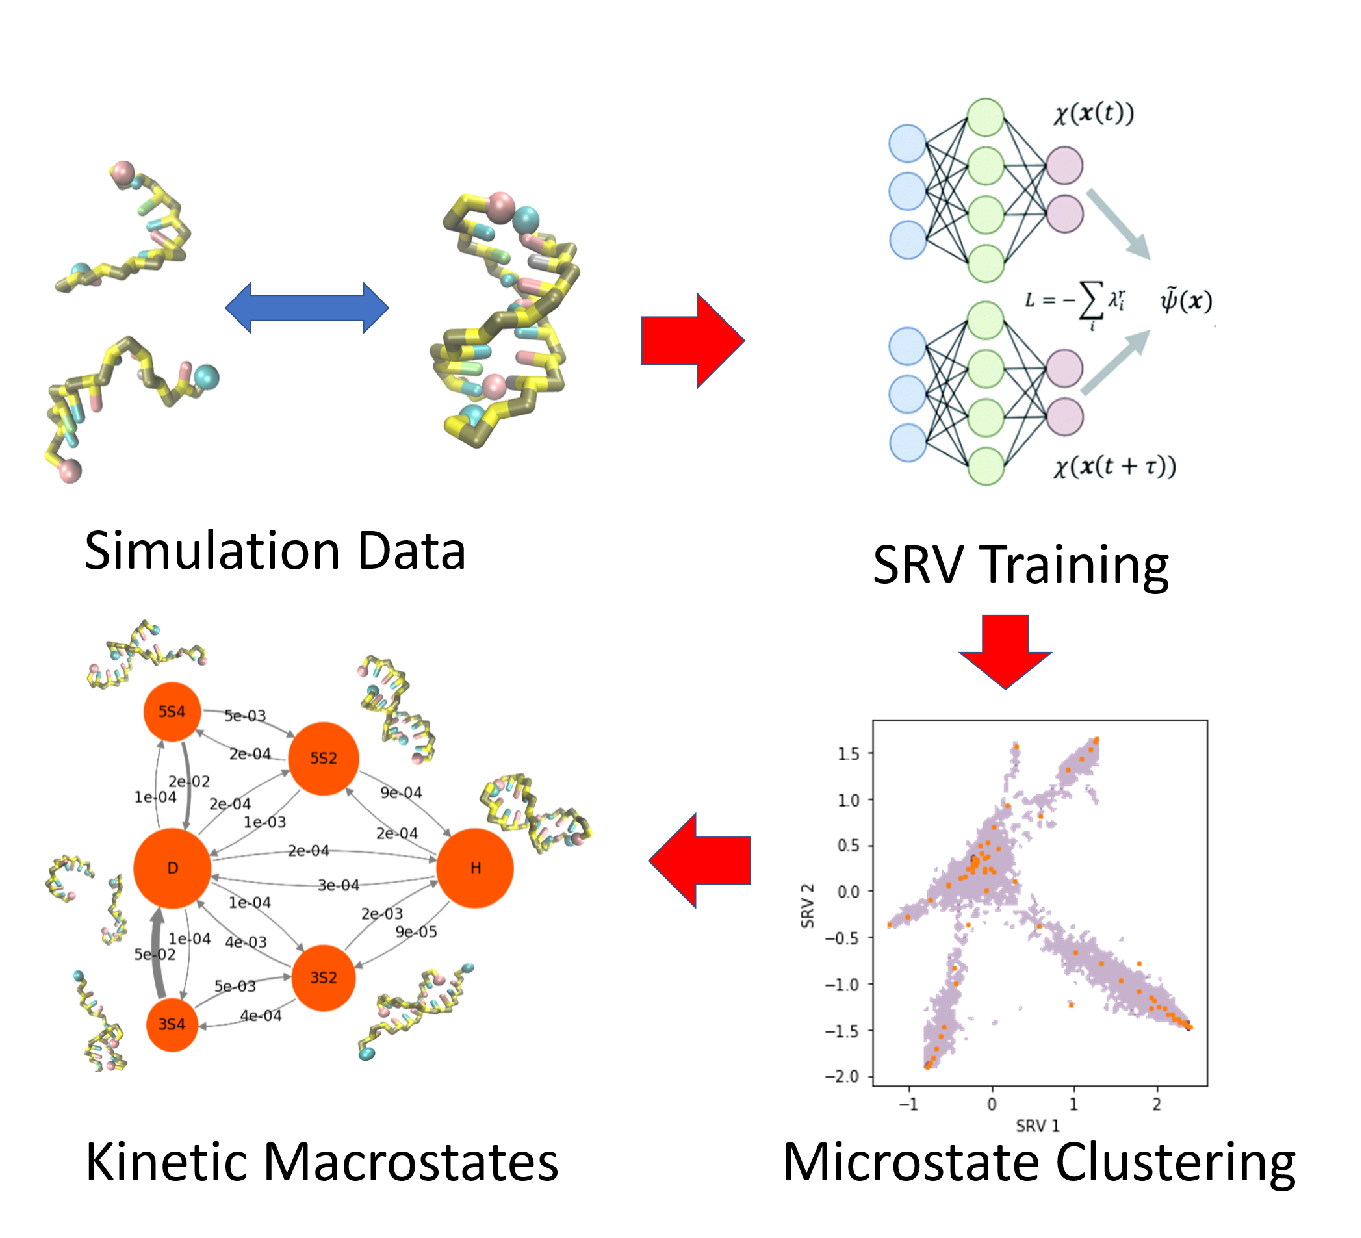
\includegraphics[width=150mm, scale=1]{TOC.pdf}
        %\caption*{For Table of Contents Only}
        \label{fig:TOC}
	\end{center}
\end{figure}

\end{document}

